\documentclass[aps,pre,reprint,floatfix,amsmath,amssymb,nofootinbib,superscriptaddress]{revtex4-2}
\usepackage{graphicx,booktabs,xcolor,url,array}
\newcolumntype{L}[1]{>{\raggedright\arraybackslash}p{#1}}
\usepackage[colorlinks=true,allcolors=blue!50!black]{hyperref}
% generated by paper/make_figures.py; do not edit
\newcommand{\awEigAW}{1.6} % studies/highk/eig.json AW K=5 Nn=128 E1=1e-2
\newcommand{\awEigSW}{\ensuremath{8\times10^{-15}}} % studies/highk/eig.json all SW points
\newcommand{\bzeroLedger}{\ensuremath{3\times10^{-18}}} % docs/_static/b00/run.json
\newcommand{\bzeroNruns}{32} % docs/_static/b00/run.json
\newcommand{\bzeroWorst}{\ensuremath{1.3\times10^{-4}}} % docs/_static/b00/run.json (Nn=128, Nx=8)
\newcommand{\cFloorHi}{757} % studies/rclosure/stagef.json
\newcommand{\cFloorLo}{713} % studies/rclosure/stagef.json
\newcommand{\cfivePicRms}{0.13} % studies/c05/run.json
\newcommand{\cgpuMax}{\ensuremath{9.7\times10^{-9}}} % studies/gpures/c08.json
\newcommand{\cohRHZ}{1.000} % studies/r1/coherence2_summary.json tau.tau30.ratio_late_mean
\newcommand{\cohRHZZ}{0.998} % studies/r1/coherence2_summary.json tau.tau300.ratio_late_mean
\newcommand{\cohROZZ}{1.089} % studies/r1/coherence2_summary.json tau.tau100.ratio_late_mean
\newcommand{\cohSeHZ}{0.007} % studies/r1/coherence2_summary.json tau.tau30.ratio_late_se
\newcommand{\cohSeHZZ}{0.003} % studies/r1/coherence2_summary.json tau.tau300.ratio_late_se
\newcommand{\cohSeOZZ}{0.064} % studies/r1/coherence2_summary.json tau.tau100.ratio_late_se
\newcommand{\dEndA}{-1.07} % recomputed from studies/r1nl/runs/pre_vq0.03_Nx32_Nn64_c64 at the window end (percent)
\newcommand{\dEndB}{-0.88} % recomputed from studies/r1nl/runs/pre_vq0.05_Nx32_Nn64_c64 at the window end (percent)
\newcommand{\dEndC}{-0.68} % recomputed from studies/r1nl/runs/pre_vq0.07_Nx32_Nn64_c64 at the window end (percent)
\newcommand{\fOneHi}{1584.5} % studies/relhhs/gates_f1.json
\newcommand{\fOneLo}{1528} % studies/relhhs/gates_f1.json
\newcommand{\fTwoPicHi}{366.5} % studies/relhhs/gates_f2.json
\newcommand{\fTwoPicLo}{265} % studies/relhhs/gates_f2.json
\newcommand{\fTwoPpc}{0.5} % studies/relhhs/gates_f2.json (npc 103)
\newcommand{\fTwoPpcStop}{160} % studies/relhhs/gates_f2.json (npc 103 positivity stop)
\newcommand{\fuDa}{\ensuremath{-1.66\times10^{-3}}} % studies/r1nl/followup_summary.json D.s1.400
\newcommand{\fuDb}{\ensuremath{-1.66\times10^{-5}}} % studies/r1nl/followup_summary.json D.s0.1.400
\newcommand{\fuDc}{\ensuremath{2.3\times10^{-9}}} % studies/r1nl/followup_summary.json D.s0.400
\newcommand{\fuFtwo}{\ensuremath{1.4\times10^{-6}}} % studies/r1nl/followup_summary.json F2
\newcommand{\fuRatio}{0.0100} % studies/r1nl/followup_summary.json F1
\newcommand{\gOneE}{\ensuremath{2.5\times10^{-9}}} % studies/relhhs/gates_g1.json
\newcommand{\gOneNR}{38} % studies/relhhs/gates_g1.json nonrel_vs_rel_W_ext (percent)
\newcommand{\gOneW}{\ensuremath{7.8\times10^{-10}}} % studies/relhhs/gates_g1.json
\newcommand{\gpuWinA}{328} % studies/gpures/summary.json
\newcommand{\gpuWinB}{595} % studies/gpures/summary.json
\newcommand{\gpuWinC}{440} % studies/gpures/summary.json
\newcommand{\gpuWinD}{751.5} % studies/gpures/summary.json
\newcommand{\hbE}{\ensuremath{1.5\times10^{-8}}} % studies/relherm/gates_b.json
\newcommand{\hbW}{\ensuremath{1.1\times10^{-8}}} % studies/relherm/gates_b.json
\newcommand{\hdLed}{\ensuremath{6.6\times10^{-10}}} % studies/relherm/gates_d.json
\newcommand{\hdTwoV}{0.83} % studies/relherm/gates_d2.json
\newcommand{\herCol}{392.5} % studies/relhhs/summary.json runs.(32, 64, 64)
\newcommand{\herColSame}{8} % studies/relhhs/summary.json (runs with collapse 392.5)
\newcommand{\herFld}{0.041} % studies/relhhs/summary.json runs.(32, 64, 64)
\newcommand{\herFldFive}{0.855} % same, t=500
\newcommand{\herHeat}{0.056} % same dE1D_e_over_Eth.1000
\newcommand{\herHeatFive}{0.018} % same, t=500
\newcommand{\herHeatMaxAll}{0.71} % studies/relhhs/summary.json (max over runs of the final averaged gain, T=1000)
\newcommand{\herLed}{\ensuremath{1.8\times10^{-8}}} % studies/relhhs/gates_prod.json (max ledger over 8 runs, t<=400)
\newcommand{\herNruns}{8} % studies/relhhs/summary.json runs
\newcommand{\hfBled}{\ensuremath{6.8\times10^{-6}}} % studies/relherm/gates_f4b.json
\newcommand{\hfOne}{\ensuremath{1\times10^{-15}}} % studies/relherm/gates_f1.json
\newcommand{\hfThree}{\ensuremath{3\times10^{-15}}} % studies/relherm/gates_f3.json (magnetic work)
\newcommand{\hfTwo}{\ensuremath{2\times10^{-10}}} % studies/relherm/gates_f2.json (gyration vs exact)
\newcommand{\hhsDEEndA}{\ensuremath{1.2\times10^{-3}}} % recomputed from studies/r1nl/runs/pre_vq0.03_Nx32_Nn64_c64 Tx, trailing 200 average, t=1000
\newcommand{\hhsDEEndB}{\ensuremath{2.3\times10^{-3}}} % recomputed from studies/r1nl/runs/pre_vq0.05_Nx32_Nn64_c64 Tx, trailing 200 average, t=892
\newcommand{\hhsDEEndC}{\ensuremath{2.5\times10^{-3}}} % recomputed from studies/r1nl/runs/pre_vq0.07_Nx32_Nn64_c64 Tx, trailing 200 average, t=791.5
\newcommand{\hhsDEVZZA}{\ensuremath{5.0\times10^{-5}}} % recomputed from studies/r1nl/runs/pre_vq0.03_Nx32_Nn64_c64 Tx, trailing 200 average, t=500
\newcommand{\hhsDEVZZB}{\ensuremath{1.4\times10^{-4}}} % recomputed from studies/r1nl/runs/pre_vq0.05_Nx32_Nn64_c64 Tx, trailing 200 average, t=500
\newcommand{\hhsDEVZZC}{\ensuremath{2.7\times10^{-4}}} % recomputed from studies/r1nl/runs/pre_vq0.07_Nx32_Nn64_c64 Tx, trailing 200 average, t=500
\newcommand{\hhsDEmaxA}{2.5} % max over the window of the averaged gain / initial thermal energy
\newcommand{\hhsDEmaxB}{4.5} % max over the window of the averaged gain / initial thermal energy
\newcommand{\hhsDEmaxC}{5} % max over the window of the averaged gain / initial thermal energy
\newcommand{\hhsDErEndA}{2.5} % same, ratio to the initial 1-D electron thermal energy
\newcommand{\hhsDErEndB}{4.5} % same, ratio to the initial 1-D electron thermal energy
\newcommand{\hhsDErEndC}{5} % same, ratio to the initial 1-D electron thermal energy
\newcommand{\hhsDErVZZA}{0.1} % same, ratio to the initial 1-D electron thermal energy
\newcommand{\hhsDErVZZB}{0.28} % same, ratio to the initial 1-D electron thermal energy
\newcommand{\hhsDErVZZC}{0.54} % same, ratio to the initial 1-D electron thermal energy
\newcommand{\hhsDigK}{50.1} % studies/relpic/digitization/hhs_fig2.json (t=1000)
\newcommand{\hhsDigKK}{52.7} % studies/relpic/digitization/hhs_fig2.json (t=2000)
\newcommand{\hhsDigRel}{3} % studies/relpic/digitization/hhs_fig2.json note (line-width uncertainty ~3 percent)
\newcommand{\hhsEth}{\ensuremath{5.0\times10^{-4}}} % v_te^2/2 with v_te^2 = 1e-3 c^2 (SM Eq. S36; HHS quote 5e-4)
\newcommand{\hhsFldEndA}{\ensuremath{4.4\times10^{-2}}} % 1/2 Ebar^2 (k=0 mean field), trailing 200 average, t=1000
\newcommand{\hhsFldEndB}{\ensuremath{9.6\times10^{-2}}} % 1/2 Ebar^2 (k=0 mean field), trailing 200 average, t=892
\newcommand{\hhsFldEndC}{\ensuremath{1.4\times10^{-1}}} % 1/2 Ebar^2 (k=0 mean field), trailing 200 average, t=791.5
\newcommand{\hhsFldLinEndA}{\ensuremath{4.6\times10^{-2}}} % same from the exact linear law
\newcommand{\hhsFldLinEndB}{\ensuremath{9.9\times10^{-2}}} % same from the exact linear law
\newcommand{\hhsFldLinEndC}{\ensuremath{1.5\times10^{-1}}} % same from the exact linear law
\newcommand{\hhsFldLinVZZA}{\ensuremath{9.2\times10^{-3}}} % same from the exact linear law
\newcommand{\hhsFldLinVZZB}{\ensuremath{2.5\times10^{-2}}} % same from the exact linear law
\newcommand{\hhsFldLinVZZC}{\ensuremath{5.0\times10^{-2}}} % same from the exact linear law
\newcommand{\hhsFldRatioA}{0.96} % mean-field energy over linear at the window end
\newcommand{\hhsFldRatioB}{0.97} % mean-field energy over linear at the window end
\newcommand{\hhsFldRatioC}{0.98} % mean-field energy over linear at the window end
\newcommand{\hhsFldVZZA}{\ensuremath{9.1\times10^{-3}}} % 1/2 Ebar^2 (k=0 mean field), trailing 200 average, t=500
\newcommand{\hhsFldVZZB}{\ensuremath{2.5\times10^{-2}}} % 1/2 Ebar^2 (k=0 mean field), trailing 200 average, t=500
\newcommand{\hhsFldVZZC}{\ensuremath{5.0\times10^{-2}}} % 1/2 Ebar^2 (k=0 mean field), trailing 200 average, t=500
\newcommand{\hhsWinTA}{1000} % last saved time within the certified window
\newcommand{\hhsWinTB}{892} % last saved time within the certified window
\newcommand{\hhsWinTC}{791.5} % last saved time within the certified window
\newcommand{\hkrHeat}{2.3} % studies/hkr/summary_grid.json Nx1024_det (nonrelativistic grid, deterministic seed)
\newcommand{\hkrK}{1.69} % studies/hkr/summary_grid.json Nx1024_det k lambda_De retained
\newcommand{\hkrNoHeat}{13.5} % studies/hkr/summary_grid.json (max 1e-3 E_th; heating at loss of positivity)
\newcommand{\hkrNoHi}{163.5} % studies/hkr/summary_grid.json
\newcommand{\hkrNoLo}{69} % studies/hkr/summary_grid.json (shot-noise runs, certified time)
\newcommand{\lawsonSteps}{5.0} % studies/expint/summary.json cases.64.steps_ratio_500
\newcommand{\lawsonStepsFour}{0.96} % studies/expint/summary.json cases.4.steps_ratio_500
\newcommand{\ledgA}{\ensuremath{7\times10^{-12}}} % studies/r1nl/stage1_summary.json vqs.0.03.ledger (max over members)
\newcommand{\ledgB}{\ensuremath{3\times10^{-12}}} % studies/r1nl/stage1_summary.json vqs.0.05.ledger (max over members)
\newcommand{\ledgC}{\ensuremath{1\times10^{-12}}} % studies/r1nl/stage1_summary.json vqs.0.07.ledger (max over members)
\newcommand{\mirA}{21.9} % studies/relpic/records/M103_s0 (dW_th/E_th, t=1000)
\newcommand{\mirB}{22.6} % studies/relpic/records/M103_s1
\newcommand{\mirC}{23.4} % studies/relpic/records/M206_s0
\newcommand{\nrColHi}{866.5} % studies/relgrid/summary.json nonrel_shot_vq0.03
\newcommand{\nrColLo}{769.5} % studies/relgrid/summary.json nonrel_shot_vq0.03
\newcommand{\nrWeakFld}{0.71} % studies/relgrid/summary.json nonrel_det_vq0.001 at t=3000
\newcommand{\nrWeakHeat}{0.22} % studies/relgrid/summary.json nonrel_det_vq0.001 at t=3000
\newcommand{\otsiMax}{1.3} % studies/instab/otsi.json scan (percent)
\newcommand{\otsiN}{22} % studies/instab/otsi.json scan
\newcommand{\pcCfive}{30.1} % studies/relpic/conv_summary.json extrapolation.C5
\newcommand{\pcCfiveU}{3.8} % studies/relpic/conv_summary.json extrapolation.C5.uncertainty
\newcommand{\pcContRatio}{445} % P1648 / relativistic Hermite dE1D_e at t=1000
\newcommand{\pcCsix}{0.60} % studies/relpic/conv_summary.json C6 ratio to HHS
\newcommand{\pcD}{21.1} % studies/relpic/conv_summary.json D (dt 0.01, ppc 103)
\newcommand{\pcF}{24.6} % studies/relpic/conv_summary.json F412 mean of 5 seeds
\newcommand{\pcFK}{28.0} % studies/relpic/conv_summary.json F412 t=2000
\newcommand{\pcFKs}{3.7} % studies/relpic/conv_summary.json F412 t=2000 std
\newcommand{\pcFldLate}{0.25} % studies/relpic/conv_summary.json F412 W_E0 at 1000 (E_th)
\newcommand{\pcFldPeak}{11} % studies/relpic/conv_summary.json F412 peak_W_E0 (E_th)
\newcommand{\pcFs}{2.0} % studies/relpic/conv_summary.json F412 seed std
\newcommand{\pcN}{62.7} % studies/relpic/conv_summary.json N412
\newcommand{\pcNK}{68.9} % studies/relpic/conv_summary.json N412 t=2000
\newcommand{\pcNewtHHS}{1.25} % studies/relpic/conv_summary.json Newtonian / HHS, t=1000
\newcommand{\pcNewtRel}{2.5} % studies/relpic/conv_summary.json Newtonian / relativistic, t=1000
\newcommand{\pcNone}{55.9} % studies/relpic/conv_summary.json N103 (ppc 103, 3 seeds)
\newcommand{\pcNs}{9.4} % studies/relpic/conv_summary.json N412 std (2 seeds)
\newcommand{\pcP}{23.7} % studies/relpic/conv_summary.json P206
\newcommand{\pcPP}{25.0} % studies/relpic/conv_summary.json P824
\newcommand{\pcPPP}{24.9} % studies/relpic/conv_summary.json P1648
\newcommand{\pcPlat}{25} % studies/relpic/conv_summary.json P1648 plateau
\newcommand{\pcPlatHHS}{0.50} % P1648 / HHS digitized, t=1000
\newcommand{\pcQ}{25.7} % studies/relpic/conv_summary.json Q412 (quintic)
\newcommand{\pcR}{21.5} % studies/relpic/conv_summary.json R103 t=1000
\newcommand{\pcRN}{0.39} % studies/relpic/conv_summary.json C7 t=1000
\newcommand{\pcRNK}{0.41} % studies/relpic/conv_summary.json C7 t=2000
\newcommand{\pcRs}{0.6} % studies/relpic/conv_summary.json R103 seed std
\newcommand{\pcStepA}{1.4} % studies/relpic/conv_summary.json change 412->824 (percent)
\newcommand{\pcStepB}{0.1} % studies/relpic/conv_summary.json change 824->1648 (percent)
\newcommand{\pcStepX}{0.8} % studies/relpic/conv_summary.json change dx 0.02->0.01 (percent)
\newcommand{\pcXa}{24.1} % studies/relpic/conv_summary.json X2 (dx 0.02)
\newcommand{\pcXb}{24.3} % studies/relpic/conv_summary.json X1 (dx 0.01)
\newcommand{\picNColHi}{311.5} % same
\newcommand{\picNColLo}{292} % studies/relpic/records N412_s0,N412_s1 (W_ext 10 percent off the exact nonrelativistic linear law)
\newcommand{\picNFldEZZ}{0.076} % studies/relpic/records N412_s0,N412_s1 mean-field energy over linear, seed mean, t=800
\newcommand{\picNFldOZZZ}{0.003} % studies/relpic/records N412_s0,N412_s1 mean-field energy over linear, seed mean, t=1000
\newcommand{\picNFldVZZ}{0.272} % studies/relpic/records N412_s0,N412_s1 mean-field energy over linear, seed mean, t=500
\newcommand{\picRColHi}{286} % same
\newcommand{\picRColLo}{273} % studies/relpic/records F412_s0,F412_s1,F412_s2,F412_s3,F412_s4 (W_ext 10 percent off the exact nonrelativistic linear law)
\newcommand{\picRFldEZZ}{0.008} % studies/relpic/records F412_s0,F412_s1,F412_s2,F412_s3,F412_s4 mean-field energy over linear, seed mean, t=800
\newcommand{\picRFldOZZZ}{0.003} % studies/relpic/records F412_s0,F412_s1,F412_s2,F412_s3,F412_s4 mean-field energy over linear, seed mean, t=1000
\newcommand{\picRFldVZZ}{0.188} % studies/relpic/records F412_s0,F412_s1,F412_s2,F412_s3,F412_s4 mean-field energy over linear, seed mean, t=500
\newcommand{\quivA}{0.47} % nonrelativistic coherent speed sqrt(2 W_ext/(n m_e)) in units of c at the window end, from pre_vq0.03_Nx32_Nn64_c64
\newcommand{\quivAtTZZ}{0.1} % v_q w_pe t/2 with v_q = 0.03 v_te, v_te^2 = 1e-3 c^2, t = 200 (units of c)
\newcommand{\quivAtVZZ}{0.2} % v_q w_pe t/2 with v_q = 0.03 v_te, v_te^2 = 1e-3 c^2, t = 500 (units of c)
\newcommand{\quivB}{0.70} % nonrelativistic coherent speed sqrt(2 W_ext/(n m_e)) in units of c at the window end, from pre_vq0.05_Nx32_Nn64_c64
\newcommand{\quivC}{0.87} % nonrelativistic coherent speed sqrt(2 W_ext/(n m_e)) in units of c at the window end, from pre_vq0.07_Nx32_Nn64_c64
\newcommand{\rOneDev}{0.039} % studies/r1/reservoir_summary.json cases.*.max_dev
\newcommand{\rOneLedger}{\ensuremath{8.4\times10^{-9}}} % studies/r1/reservoir_summary.json gates.G1_ledger_max
\newcommand{\recomputeWext}{381.3} % recomputed from studies/r1nl/runs/pre_vq0.07_Nx32_Nn64_c64 (check vs rnlWext)
\newcommand{\relColGrid}{392} % studies/relgrid/summary.json cases.rel_det_vq0.03.t_W_10pc_from_linear
\newcommand{\relColShotHi}{392.5} % studies/relgrid/summary.json rel_shot_vq0.03 npc>=2.05e4
\newcommand{\relColShotLo}{367} % studies/relgrid/summary.json rel_shot_vq0.03 npc>=2.05e4
\newcommand{\relColWeak}{1309.5} % studies/relgrid/summary.json rel_det_vq0.001
\newcommand{\relColWeakShot}{1413.5} % studies/relgrid/summary.json rel_shot_vq0.001
\newcommand{\relFldAbsGrid}{3.7} % studies/relgrid/summary.json Ebar_energy.1000 / E_th
\newcommand{\relFldAbsN}{\ensuremath{1.9\times10^{-3}}} % studies/relgrid/summary.json Ebar_energy.1000 (n m c^2)
\newcommand{\relFldGrid}{0.041} % studies/relgrid/summary.json cases.rel_det_vq0.03.Ebar_energy_over_linear.1000
\newcommand{\relFldGridFive}{0.85} % studies/relgrid/summary.json same, t=500
\newcommand{\relHeatGrid}{0.056} % studies/relgrid/summary.json same dE1D_over_Eth.1000
\newcommand{\relHomWratio}{0.0056} % studies/relgrid/summary.json homog.vq0.03 (exact homogeneous ODEs, rel/nonrel W_ext at t=1000)
\newcommand{\relWeakFld}{0.50} % studies/relgrid/summary.json rel_det_vq0.001 at t=3000
\newcommand{\relWeakHeat}{0.09} % studies/relgrid/summary.json rel_det_vq0.001 at t=3000
\newcommand{\rgCerrG}{\ensuremath{4.5\times10^{-4}}} % studies/relgrid/gates_c2.json (max err_gamma)
\newcommand{\rgCerrW}{\ensuremath{8.9\times10^{-5}}} % studies/relgrid/gates_c2.json (max err_omega, k lambda_De=0.3,0.4)
\newcommand{\rgDfail}{15} % studies/relgrid/summary.json gate_D (runs failing the 1e-4 ledger)
\newcommand{\rgDled}{\ensuremath{2.3\times10^{-4}}} % studies/relgrid/summary.json gate_D (dt 0.02)
\newcommand{\rgDledOne}{\ensuremath{2.9\times10^{-5}}} % studies/relgrid/summary.json gate_D (dt 0.01)
\newcommand{\rgDratio}{8.0} % studies/relgrid/summary.json gate_D ledger ratio dt 0.02 / 0.01
\newcommand{\rgDtot}{16} % studies/relgrid/summary.json gate_D runs
\newcommand{\rnlBound}{0.68} % studies/r1nl/stage2_summary.json N1.bound_max_abs_D (percent)
\newcommand{\rnlCohShare}{97} % studies/r1nl/stage2_summary.json N3.B.dKe / N1.Wext (percent)
\newcommand{\rnlDKe}{371} % studies/r1nl/stage2_summary.json N3.B
\newcommand{\rnlDw}{\ensuremath{6.5\times10^{-6}}} % studies/r1nl/stage2_summary.json N2.bound
\newcommand{\rnlEtaO}{0.049} % stage2_summary.json N4.u1.eta
\newcommand{\rnlEtaOZ}{0.016} % stage2_summary.json N4.u10.eta
\newcommand{\rnlFluct}{2077} % studies/r1nl/stage2_summary.json N3.B
\newcommand{\rnlIonShare}{0.05} % studies/r1nl/stage2_summary.json N3.B (percent)
\newcommand{\rnlLedger}{\ensuremath{1.7\times10^{-9}}} % studies/r1nl/stage2_summary.json N6
\newcommand{\rnlNruns}{33} % studies/r1nl/stage2_summary.json N6
\newcommand{\rnlOtsi}{783.5} % studies/r1nl/stage2_summary.json N3.B.t_otsi
\newcommand{\rnlOtsiN}{862} % studies/r1nl/stage2_summary.json N3.N.t_otsi
\newcommand{\rnlRHZZ}{1.0000} % stage2_summary.json N5.tau300.R
\newcommand{\rnlROZZ}{1.0050} % stage2_summary.json N5.tau100.R
\newcommand{\rnlRbHZZ}{0.8} % stage2_summary.json N5.tau300.bound_if_none (percent)
\newcommand{\rnlRbOZZ}{1.7} % stage2_summary.json N5.tau100.bound_if_none (percent)
\newcommand{\rnlResO}{0.23} % stage2_summary.json N4.u1 (percent of U_D0)
\newcommand{\rnlResOZ}{0.81} % stage2_summary.json N4.u10 (percent of U_D0)
\newcommand{\rnlResWO}{1.0} % stage2_summary.json N4.u1 (percent)
\newcommand{\rnlResWOZ}{2.7} % stage2_summary.json N4.u10 (percent)
\newcommand{\rnlRmaxHZZ}{1.5} % stage2_summary.json N5.tau300 (percent of peak W_lin)
\newcommand{\rnlRmaxOZZ}{4.7} % stage2_summary.json N5.tau100 (percent of peak W_lin)
\newcommand{\rnlRseHZZ}{0.0038} % stage2_summary.json N5.tau300.se
\newcommand{\rnlRseOZZ}{0.0058} % stage2_summary.json N5.tau100.se
\newcommand{\rnlSplitO}{50.5} % stage2_summary.json N4.u1.t_split_kin
\newcommand{\rnlSplitOZ}{72} % stage2_summary.json N4.u10.t_split_kin
\newcommand{\rnlSpread}{\ensuremath{2\times10^{-4}}} % studies/r1nl/stage2_summary.json N1.max_abs_D_by_member
\newcommand{\rnlWDfrac}{47} % stage2_summary.json N4.u1 (percent of U_D0 given up)
\newcommand{\rnlWext}{381.3} % studies/r1nl/stage2_summary.json N1
\newcommand{\rnlWlin}{384.0} % studies/r1nl/stage2_summary.json N1
\newcommand{\rtwoCV}{36} % studies/r2/summary.json counts.CV
\newcommand{\rtwoCVN}{36} % studies/r2/summary.json counts.CV
\newcommand{\rtwoCVwx}{\ensuremath{2.5\times10^{-6}}} % studies/r2/summary.json cases.*.B.CV.Wx
\newcommand{\rtwoDetH}{9} % studies/r2/summary.json detuned nu=1e-3 mean R_late - 1 (percent)
\newcommand{\rtwoDetHi}{14} % studies/r2/summary.json detuned nu=1e-3 R_late (percent)
\newcommand{\rtwoDetL}{14} % studies/r2/summary.json detuned nu=1e-3 mean R_late - 1 (percent)
\newcommand{\rtwoDetLo}{8} % studies/r2/summary.json detuned nu=1e-3 R_late (percent)
\newcommand{\rtwoFuA}{0.0105} % studies/r2/followup_summary.json
\newcommand{\rtwoFuB}{0.0099} % studies/r2/followup_summary.json
\newcommand{\rtwoKH}{1.025} % studies/r2/summary.json fits.1.1.kappa
\newcommand{\rtwoKL}{1.040} % studies/r2/summary.json fits.0.9.kappa
\newcommand{\rtwoKR}{0.985} % studies/r2/summary.json fits.res.kappa
\newcommand{\rtwoKeH}{0.011} % studies/r2/summary.json fits.1.1.kappa_se
\newcommand{\rtwoKeL}{0.017} % studies/r2/summary.json fits.0.9.kappa_se
\newcommand{\rtwoKeR}{0.003} % studies/r2/summary.json fits.res.kappa_se
\newcommand{\rtwoKthree}{12} % studies/r2/summary.json counts.K3
\newcommand{\rtwoKthreeN}{12} % studies/r2/summary.json counts.K3
\newcommand{\rtwoKtwo}{30} % studies/r2/summary.json counts.K2
\newcommand{\rtwoKtwoN}{36} % studies/r2/summary.json counts.K2
\newcommand{\rtwoPH}{2.00} % studies/r2/summary.json fits.1.1.kin.p
\newcommand{\rtwoPL}{2.00} % studies/r2/summary.json fits.0.9.kin.p
\newcommand{\rtwoPR}{1.99} % studies/r2/summary.json fits.res.kin.p
\newcommand{\rtwoPeH}{0.02} % studies/r2/summary.json fits.1.1.kin.se_p
\newcommand{\rtwoPeL}{0.03} % studies/r2/summary.json fits.0.9.kin.se_p
\newcommand{\rtwoPeR}{0.10} % studies/r2/summary.json fits.res.kin.se_p
\newcommand{\rtwoPss}{0.4} % studies/r2/summary.json cases.*nu0.03*.B.P_kin_over_pss (percent)
\newcommand{\rtwoQH}{0.88} % studies/r2/summary.json fits.1.1.kin.q
\newcommand{\rtwoQL}{0.75} % studies/r2/summary.json fits.0.9.kin.q
\newcommand{\rtwoQR}{-0.51} % studies/r2/summary.json fits.res.kin.q
\newcommand{\rtwoQeH}{0.01} % studies/r2/summary.json fits.1.1.kin.se_q
\newcommand{\rtwoQeL}{0.02} % studies/r2/summary.json fits.0.9.kin.se_q
\newcommand{\rtwoQeR}{0.05} % studies/r2/summary.json fits.res.kin.se_q
\newcommand{\rtwoQlH}{0.90} % studies/r2/summary.json fits.1.1.lin.q
\newcommand{\rtwoQlL}{0.79} % studies/r2/summary.json fits.0.9.lin.q
\newcommand{\rtwoQlR}{-0.52} % studies/r2/summary.json fits.res.lin.q
\newcommand{\rtwoResHi}{0.9979} % studies/r2/summary.json
\newcommand{\rtwoResLo}{0.963} % studies/r2/summary.json
\newcommand{\rtwoTmax}{231} % studies/r2/summary.json cases.*.B.report
\newcommand{\shotFnegHi}{407.5} % studies/relgrid/summary.json rel_shot_vq0.03 first f<-1e-3 (npc>=2.05e4)
\newcommand{\shotFnegLo}{240.5} % studies/relgrid/summary.json rel_shot_vq0.03 first f<-1e-3 (npc>=2.05e4)
\newcommand{\shotFnegPic}{0.5} % studies/relgrid/summary.json rel_shot_vq0.03_npc205_Nx32 first f<-1e-3 (205 per cell = PIC particle number)
\newcommand{\shotHeatNx}{5.4} % studies/relgrid/summary.json Nx64 npc 2.05e5 at t=500 (invalid)
\newcommand{\wextA}{111} % recomputed from studies/r1nl/runs/pre_vq0.03_Nx32_Nn64_c64 at the window end, units n T_e V
\newcommand{\wextB}{247} % recomputed from studies/r1nl/runs/pre_vq0.05_Nx32_Nn64_c64 at the window end, units n T_e V
\newcommand{\wextC}{381} % recomputed from studies/r1nl/runs/pre_vq0.07_Nx32_Nn64_c64 at the window end, units n T_e V
\newcommand{\winA}{1000} % studies/r1nl/stage1_summary.json vqs.0.03.window
\newcommand{\winB}{892} % studies/r1nl/stage1_summary.json vqs.0.05.window
\newcommand{\winC}{791.5} % studies/r1nl/stage1_summary.json vqs.0.07.window

% generated by paper/make_figures.py; do not edit
\newcommand{\tabWindows}{%
\begin{tabular}{@{}lcccc@{}}\toprule
$v_q/v_{te}$ & window $\omega_{pe}t$ & limiter & $\max$ ledger (B) & grid agrees with B until\\\midrule
0.03 & 1000 & cap $T=1000$ & $6.6\times10^{-12}$ & 1000 / 1000\\
0.05 & 892 & positivity, $N_x=64$ & $3.3\times10^{-12}$ & 979.5 / 962.5\\
0.07 & 791.5 & positivity, $N_x=64$ & $9.7\times10^{-13}$ & 870 / 863\\
\bottomrule\end{tabular}}
\newcommand{\tabRtwo}{%
\begin{tabular}{@{}llccccc@{}}\toprule
$\omega/\omega_{pe}$ & $\nu_{ei}/\omega_{pe}$ & $P_{\rm lin}/P_{\rm ss}$ & $P_{\rm kin}/P_{\rm ss}$ & $P_{\rm kin}/P_{\rm lin}$ & $T_e/T_e(0)$ & 5\,\% check\\\midrule
res. & 0.001 & 0.20 & 0.192 & 0.9830 & 35.2 & pass\\
res. & 0.003 & 0.48 & 0.472 & 0.9841 & 68.6 & pass\\
res. & 0.01 & 0.89 & 0.877 & 0.9908 & 83.6 & pass\\
res. & 0.03 & 1.00 & 0.996 & 0.9979 & 48.1 & pass\\
\addlinespace
0.9 & 0.001 & 2.00 & 2.279 & 1.1406 & 1.02 & FAIL\\
0.9 & 0.003 & 1.54 & 1.584 & 1.0281 & 1.05 & pass\\
0.9 & 0.01 & 1.11 & 1.106 & 0.9994 & 1.12 & pass\\
0.9 & 0.03 & 1.00 & 1.003 & 1.0000 & 1.32 & pass\\
\addlinespace
1.1 & 0.001 & 1.38 & 1.496 & 1.0857 & 1.02 & FAIL\\
1.1 & 0.003 & 1.21 & 1.224 & 1.0145 & 1.05 & pass\\
1.1 & 0.01 & 1.04 & 1.037 & 0.9996 & 1.14 & pass\\
1.1 & 0.03 & 1.00 & 1.000 & 1.0000 & 1.38 & pass\\
\bottomrule\end{tabular}}
\newcommand{\tabVerify}{%
\begin{tabular}{@{}L{5.6cm}L{10.4cm}@{}}\toprule
Check & Result (record)\\\midrule
Linear Landau roots, ordinary and dark, $k\lambda_{De}=0.2$--$0.7$ & worst relative error $1.3\times10^{-4}$ vs.\ SciPy Faddeeva roots; ledger defect $\le$ $3\times10^{-18}$\\
OTSI growth vs.\ Silin kinetic relation (sideband determinant) & 22 unstable points, worst difference 1.3\%\\
Dark-JAX-in-Cell PIC, Landau $k\lambda_{De}=0.5$ & rms $\Delta\ln|E_k|$ falls 0.22$\to$0.13 from 32 to 128 cells; PIC noise limits agreement to $\sim$1\%\\
GPU vs.\ CPU, one case ($T=100$) & max relative difference $9.7\times10^{-9}$ (adaptive trajectories)\\
% numbers: studies/c09/run.json
AD vs.\ finite differences & reverse = forward to $2\times10^{-13}$, analytic to $5\times10^{-10}$ (19 derivatives)\\
\bottomrule\end{tabular}}
\newcommand{\tabSeed}{%
\begin{tabular}{@{}lcccc@{}}\toprule
seed scale $s$ & $D(100)$ & $D(200)$ & $D(300)$ & $D(400)$\\\midrule
1 & $-1.03\times10^{-4}$ & $-4.15\times10^{-4}$ & $-9.35\times10^{-4}$ & $-1.66\times10^{-3}$\\
0.1 & $-1.03\times10^{-6}$ & $-4.15\times10^{-6}$ & $-9.36\times10^{-6}$ & $-1.66\times10^{-5}$\\
0 (unseeded) & $1.00\times10^{-10}$ & $8.58\times10^{-10}$ & $1.58\times10^{-9}$ & $2.27\times10^{-9}$\\
\bottomrule\end{tabular}}
\newcommand{\tabRel}{%
\begin{tabular}{@{}L{3.6cm}cccc@{}}\toprule
model & collapse time & $\bar E^2/2$ over linear, $t=1000$ & $\Delta E_e/E_{\rm th}$, $t=1000$ & valid to\\\midrule
Hermite, nonrel.\ ($N_x=32,N_n=64$) & none ($\le1000$) & \hhsFldRatioA & \hhsDErEndA & \winA\\
grid, nonrel., shot noise$^{\dagger}$ & \nrColLo--\nrColHi & 0.12--0.26 & 99--209 & 240--394\\
grid, rel., deterministic & \relColGrid & \relFldGrid & \relHeatGrid & 1000\\
Hermite, rel., deterministic & \herCol & \herFld & \herHeat & \fOneLo--\fOneHi\\
grid, rel., shot noise$^{\dagger}$ & \relColShotLo--\relColShotHi & 0.008--0.30 & 15--51 & \shotFnegLo--\shotFnegHi\\
\addlinespace
PIC, rel.\ (ppc 412) & \picRColLo--\picRColHi & \picRFldOZZZ & \pcF & ---\\
PIC, Newtonian (ppc 412) & \picNColLo--\picNColHi & \picNFldOZZZ & \pcN & ---\\
HHS (digitized) & loss of resonance $\sim800$ & --- & \hhsDigK & ---\\
\bottomrule\end{tabular}}

\newcommand{\vq}{v_q/v_{te}}
\newcommand{\nTV}{nT_eV}
\newcommand{\wpe}{\omega_{pe}}
\newcommand{\Wext}{W_{\rm ext}}
\newcommand{\Wlin}{W_{\rm lin}}

\setlength{\emergencystretch}{3em}
\setlength{\textfloatsep}{10pt plus 2pt minus 4pt}
\setlength{\floatsep}{8pt plus 2pt minus 2pt}
\begin{document}
\title{Resonant conversion of dark-photon fields in a plasma with a noise-free continuum kinetic method: bounds on nonlinear suppression and the role of collisions}
\author{Rogerio Jorge}
\email{rogerio.jorge@wisc.edu}
\affiliation{Department of Physics, University of Wisconsin--Madison, Madison, Wisconsin 53706, USA}
\date{\today}

\begin{abstract}
Particle-in-cell simulations have been argued to show that nonlinear plasma dynamics cuts off the resonant conversion of dark-photon dark matter into plasma oscillations in the early Universe (Hook, Huang and Shalaby). We test this with a noise-free Hermite--Fourier Vlasov solver for the nonrelativistic Maxwell--Proca--Vlasov system with kinetic mixing, in one spatial and three velocity dimensions. The method is limited by a truncation instability of the asymmetrically weighted Hermite basis, which bounds the certified windows (the times over which refinement, positivity and energy-ledger checks pass) to \winA, \winB\ and \winC\ in units of $\wpe^{-1}$ at drive strengths $\vq=0.03$, 0.05 and 0.07; the alternative bases and closures we tested did not remove it. Inside the windows, at $\vq=0.07$ the energy transfer follows the linear resonant law to \rnlBound\,\% with no resolved frequency detuning (bound \rnlDw\ $\wpe$). A finite dark reservoir and a finite coherence time of the drive leave the linear prediction unchanged to \rnlResOZ\,\% of the initial reservoir energy and \rnlRbOZZ\,\% of the ensemble work. With collisions, the kinetic absorption equals the linear Drude law with $\nu_{\rm eff}=(\nu_{ei}/2)(1+m_e/m_i)$: the late rate is within \rtwoPss\,\% of the steady-state power at $\nu_{ei}=3\times10^{-2}\wpe$, and the work scales as $(\vq)^{p}$ with $p=\rtwoPR\pm\rtwoPeR$. At the one drive that matches a published particle-in-cell run ($\vq=0.03$), our electron $k\ne0$ energy is \hhsDErVZZA\ initial thermal energies at $\wpe t=500$ and \hhsDErEndA\ at $\wpe t=1000$, against about 50 reported there, and the mean-field energy stays at \hhsFldRatioA\ of the linear value: we do not reproduce the saturation at the matched drive. The model is nonrelativistic, whereas the coherent quiver speed reaches \quivA$c$ at that drive and \quivC$c$ at the strongest; relativistic detuning, absent here, is an untested candidate for the difference. These are bounds in a restricted model, not a resolution of the cosmological question: they hold in one dimension for $\vq\le0.07$ and $\wpe t\lesssim790$ at the strongest drive, before the oscillating two-stream cascade develops.
\end{abstract}
\maketitle

\section{Introduction}
A dark photon with kinetic mixing $\chi$ with the ordinary photon and a mass $m_{A'}$ is a well-motivated candidate for dark matter~\cite{Fabbrichesi2020}. In the early Universe the dark-photon field oscillates coherently, and when $m_{A'}$ equals the plasma frequency of the ionized medium the field resonantly converts into longitudinal plasma oscillations, depositing energy in the plasma~\cite{DubovskyHC2015,McDermottWitte2020,Witte2020}. Cosmological constraints on dark-photon dark matter have been derived from the resonant transfer of a substantial part of the dark-photon energy density into the plasma, which heats it.

Hook, Huang and Shalaby (HHS) argued that the resonant transfer saturates because of plasma nonlinearities~\cite{HHS2026}. In their account, large-amplitude $k\simeq0$ Langmuir waves, driven by the dark photon, excite higher-$k$ Langmuir and ion-acoustic waves through the ponderomotive force; the resulting density inhomogeneities detune the resonance and limit the deposited energy to roughly the electron thermal energy, which would weaken the constraints by several orders of magnitude. Their evidence comes from one-dimensional particle-in-cell (PIC) simulations (SHARP, with a relativistic Vay pusher) of an electron--ion plasma with $m_i/m_e=1836$ and a prescribed uniform dark-photon drive: resonant runs at $v_q^D/v_{th}^e=0.03$ and $10^{-3}$ (their Fig.~2) and Landau--Zener runs (their Fig.~3), published as Phys.\ Rev.\ Lett.\ 137, 071004. They quote a saturation of the energy transfer at roughly the electron thermal energy for weak drives and up to about $10^2$ times it for strong ones.

A PIC calculation carries sampling noise, which seeds the very instabilities that the argument relies on. This paper asks a narrow question and answers it with a different numerical method: in a model with the same physical ingredients, when does the energy transfer from a resonant uniform drive depart from the linear resonant law, and how large is the departure that can be resolved? We write $\vq\equiv E_0/(v_{te}\wpe)$ for the drive strength, with $E_0$ the drive amplitude, $v_{te}$ the electron thermal speed and $\wpe$ the electron plasma frequency (Sec.~\ref{sec:units}). We use a noise-free continuum kinetic solver whose seeds are deterministic and whose work ledger closes to solver tolerance, so that any departure from the linear law can be attributed. We do not reproduce the HHS simulations: our model is nonrelativistic, the loading is deterministic, and the box and parameters differ in detail; Sec.~\ref{sec:hhs} states which of our numbers are comparable to theirs and which are not.

The work consists of a methods part and a bounds part. The methods part (Secs.~\ref{sec:model}--\ref{sec:verify}) describes the model, the Hermite--Fourier discretization, the verification suite, and the failure mode that limits the method. The results part addresses two research questions: (i) does a finite dark-photon reservoir or a finite coherence time of the drive produce detuning or saturation of the energy transfer at the strongest drives we can certify (Sec.~\ref{sec:r1})? and (ii) with collisions present, does the sustained absorption obey the linear drag law, and what is missing before a cosmological statement (Sec.~\ref{sec:r2})? Failed and amended checks are reported where they affect a claim.

\section{Model}\label{sec:model}
\subsection{Canonical Maxwell--Proca--Vlasov system}
Each species $s$ obeys the collisionless Vlasov equation in the combined force field,
\begin{multline}
\partial_t f_s+\mathbf v\!\cdot\!\nabla f_s+\frac{q_s}{m_s}\Big[\mathbf E+\eta\mathbf E_D+\mathbf E_{\rm drive}\\+\mathbf v\times(\mathbf B+\eta\mathbf B_D)\Big]\!\cdot\!\nabla_v f_s=0 ,
\end{multline}
with ordinary fields $\partial_t\mathbf E=c^2\nabla\times\mathbf B-\mathbf J/\epsilon_0$, $\partial_t\mathbf B=-\nabla\times\mathbf E$ and canonical Proca fields
\begin{align}
\partial_t\mathbf E_D&=c^2\nabla\times\mathbf B_D+\Omega_D^2\mathbf A_D-\eta\mathbf J/\epsilon_0,\\
\partial_t\mathbf B_D&=-\nabla\times\mathbf E_D,\quad
\partial_t\mathbf A_D=-\mathbf E_D-\nabla\phi_D,\\
\partial_t\phi_D&=-c^2\nabla\!\cdot\!\mathbf A_D ,
\end{align}
with constraints $\nabla\!\cdot\!\mathbf E=\rho/\epsilon_0$ and $\nabla\!\cdot\!\mathbf E_D+\Omega_D^2\phi_D/c^2=\eta\rho/\epsilon_0$. The ordinary current $\mathbf J$ sources both laws; the dark field acts back on the particles with strength $\eta$. Three modes are used: \emph{ordinary} (no dark coupling), \emph{prescribed drive} (a uniform $\mathbf E_{\rm drive}=\mathbf E_0\cos(\omega t+\varphi)$ and an external-work ledger, no dark reservoir; the setting of HHS), and \emph{self-consistent} (evolved Proca fields with a finite energy reservoir).

\subsection{Mixing map}
For a kinetic mixing $-\tfrac{\chi}{2}F_{\mu\nu}F_D^{\mu\nu}$ and a mass term on the dark field only, removing the mixing by a non-orthogonal shear gives the canonical coupling
\begin{equation}
\eta=\frac{\chi}{\sqrt{1-\chi^2}},\qquad m_D=\frac{m_0}{\sqrt{1-\chi^2}},
\end{equation}
where $m_0$ is the bare mass and $\Omega_D$ is the dark-photon mass $m_D$ expressed as a frequency. We checked this map against Sec.~1.1 of Ref.~\cite{Fabbrichesi2020} (their $\varepsilon\equiv\chi$): the dark photon couples to the ordinary current with strength $e\varepsilon/\sqrt{1-\varepsilon^2}$. The sign convention differs by $\mathbf A_D\to-\mathbf A_D$, under which the model is symmetric in $\eta$. The model is not the massless ``millicharged'' choice of the same reference.

\subsection{Energy and work ledger}
In the parent normalization velocities are in units of $c$, $\Omega_0\equiv\Omega_{c,0}$ and the species mass is $m_s=\Omega_0/\Omega_{cs}$, which is required for the energy theorem. With $\langle\cdot\rangle$ the box average the field energies and powers are
\begin{align}
U_\gamma&=\tfrac12\Omega_0^2\langle E^2+B^2\rangle,\\
U_D&=\tfrac12\Omega_0^2\big\langle E_D^2+B_D^2+\Omega_D^2(A_D^2+\phi_D^2)\big\rangle,\\
P_\gamma&=\Omega_0\langle\mathbf J\!\cdot\!\mathbf E\rangle,\quad
P_D=\Omega_0\eta\langle\mathbf J\!\cdot\!\mathbf E_D\rangle,\\
P_{\rm ext}&=\Omega_0\bar{\mathbf J}\!\cdot\!\mathbf E_{\rm drive}.
\end{align}
The works $W_\gamma$, $W_D$, $\Wext$ are integrated as extra ODE states with the same Runge--Kutta stages as the fields, so that $K-K_0=W_\gamma+W_D+\Wext$, $U_\gamma-U_{\gamma0}=-W_\gamma$ and $U_D-U_{D0}=-W_D$ hold to solver tolerance. The Proca energy flux is $\epsilon_0c^2\mathbf E_D\times\mathbf B_D+\epsilon_0\Omega_D^2\phi_D\mathbf A_D$; omitting the $\phi_D\mathbf A_D$ term breaks the flux budget (Sec.~\ref{sec:verify}). For a homogeneous plasma under the uniform drive the mean field obeys a driven oscillator at the plasma frequency $\omega_L=\sqrt{1+m_e/m_i}\,\wpe$, whose solution is the \emph{linear resonant law}: $\dot{\bar E}=-\bar J$, $\dot{\bar J}=\omega_L^2(\bar E+E_0\cos\omega t)$, $\dot W=\bar J E_0\cos\omega t$. This law is exact in the homogeneous discrete Hermite system because only Hermite orders 0--1 enter (a homogeneous check, agreement to $10^{-9}$ for $\wpe t\le1000$ even at quiver speeds of 15\,$v_{te}$). With fluctuations present it is the baseline against which the transfer is measured, and the departure from it contains the $\langle\delta n\,\delta E\rangle$ back-reaction term of the mean-field identity.

\subsection{Units and the HHS-like set-up}\label{sec:units}
All simulations use $c=\wpe=n=1$ for the electrons, $m_i/m_e=1836$, $T_i=T_e$, $v_{te}^2=10^{-3}c^2$, box length $L=40\,c/\wpe$ and a prescribed drive at $\omega=\omega_L$ unless stated. We call $\vq\equiv E_0/(v_{te}\wpe)$ the effective initial force (the quiver speed grows secularly with time at resonance). Energies are quoted in units of $\nTV$. HHS use $v_q^D/v_{th}^e=0.03$ and $10^{-3}$ for their resonant runs (PRL Fig.~2), $m_i/m_e=1836$, $k_BT_e=k_BT_i=10^{-3}m_ec^2$ ($v_{th}^e=3.1\times10^{-2}c$), $L=40\,c/\wpe$ with 1000 cells of $0.04\,c/\wpe$ and a prescribed spatially uniform drive $A_0\cos\omega t$ (Supplemental Material, Sec.~II); we use the same $v_{te}$, mass ratio, temperature ratio, box length and $v_q$ definition, but not the loading (their particles start equally spaced, ions and electrons colocated; ours is a deterministic spectral seed) or the relativistic pusher. Runs here are \emph{HHS-inspired}, not reproductions.

\section{Method}\label{sec:method}
\subsection{Hermite--Fourier discretization}
The velocity dependence is expanded in Cartesian asymmetrically weighted (AW) Hermite functions with independent orders $(N_n,N_m,N_p)$, widths $\alpha_s$ and centres $u_s$; space is Fourier, with the strict $2/3$ dealiasing mask of the parent (which retains $3|m|<N_x$, so every grid size is alias-free for quadratic products). A single call to the SPECTRAX Hermite--Fourier kernel per right-hand-side evaluation receives the physical force fields $\mathbf E+\eta\mathbf E_D+\mathbf E_{\rm drive}$ and $\mathbf B+\eta\mathbf B_D$, and the current is evaluated once for both Amp\`ere laws. Time integration is Dopri8 with a PID controller (Diffrax). The kinetic-energy ledger closes only when every forced direction has Hermite order at least 3. The parent is SPECTRAX~\cite{SPECTRAX}; the studies reported here were run at the parent commits recorded in each record, all on an unmerged integration branch of open parent changes, not a release (see Data and code availability).

\subsection{Pump frame and basis remaps}
In the pump frame the state carries the centres $u_s$ and widths $\alpha_s$. Each centre follows the total uniform force, $\dot u_s=(q/m)_s(\bar{\mathbf E}+u_s\times\bar{\mathbf B})$, with the box averages including $\eta\mathbf E_D$ and the drive; the parent kernel then uses $\mathbf E-\bar{\mathbf E}$. This is an exact change of variables: the coherent $k=0$ quiver sits in $u_s(t)$ rather than in high Hermite orders. Widths and residual drifts change only between integration segments, through the parent's exact lower-triangular remap (every moment below the truncation is preserved); triggers fire on $|U-u|/a>0.3$ or $|a'/a-1|>0.05$, with caps $|\Delta u|\le a'$, $a/a'\le1.1$, $a'\ge1.1\sigma$.

\subsection{Closures}
Truncation needs a closure. The parent closure is a hypercollision $\propto n(n-1)(n-2)$ that leaves Hermite orders 0--2 unchanged. We use a field-scaled form, implemented in the SPECTRAX integration branch,
\begin{multline}
\nu_s=c\,\Big|\frac{q}{m}\Big|_s\frac{\sqrt{2N_n}\,\max|E-\langle E\rangle|}{a_s}\\\times\frac{n(n-1)(n-2)}{(N_n-1)(N_n-2)(N_n-3)},
\end{multline}
with strength $c$ (density, momentum and energy rows untouched; a Lorentz-force-scaled variant exists for magnetized runs and is not needed here). For $c=64$ the closure rate is the stiff eigenvalue of the system: the Jacobian's spectral radius equals the closure rate $\nu_e$ (real and negative) to the printed precision, so the explicit step is bounded by $5.17/\nu_e$. We therefore integrate the diagonal closure damping exactly with a Lawson integrating factor~\cite{Lawson1967} wrapped around Dopri8 (integrating-factor and exponential Runge--Kutta methods are reviewed in Ref.~\cite{Hochbruck2010}, and for kinetic equations in Ref.~\cite{Crouseilles2020}). Lawson transforms $y'=f(t,y)$ with a matrix $A$ by $z=e^{-tA}y$ and advances $z$ with an explicit Runge--Kutta method, so that the stiff part of the Jacobian, $e^{-tA}(\partial f/\partial y)e^{tA}-A$, is removed from the step-size restriction; $A$ may be re-evaluated at each step from the local Jacobian (his Algorithm~II)~\cite{Lawson1967}. Here $A=-\mathrm{diag}(r)$ is the closure rate frozen at the step start, so with $w=e^{r(t-t_0)}y$ the split is an identity within the step; streaming, the force, the fields and the variation of $\nu$ over the step stay explicit. Lawson shows that the construction is A-stable for the linear test problem if the exponential is approximated stably, is stable for $y'=By+u(t,y)$ when the Lipschitz constant of $u$ is small compared with the spectral radius of $B$, and keeps the order of the underlying Runge--Kutta method when $\exp(hA)$ is approximated to at least that order~\cite{Lawson1967}; here the diagonal exponential is exact. These statements hold for $h\to0$ at fixed $A$. For semilinear problems with large $A$, Hochbruck and Ostermann show that the stiff order of such methods can be lower than the classical one (the Lawson--Runge scheme is only first-order accurate under their stiff-order theory, Example~2.32 and Theorem~2.17 of Ref.~\cite{Hochbruck2010}), so we do not claim that the order of Dopri8 is retained when $rh\gg1$; we rely on the measured agreement with the unfactored integration instead. For $c=64$ the factor reduces the step count by a factor \lawsonSteps\ to $t=500$ with $\Delta K_e$ and $\Wext$ agreeing with the Dopri8 record to $5\times10^{-10}$; for $c=4$, where the closure is not stiff, it gives \lawsonStepsFour\ (no gain). An exact Hermite-streaming factor was also built and rejected: it gave no step reduction and cost 2.7 times more per step. Table~\ref{tab:failed} lists these and other negative results.

\subsection{Collisions}
Collisions use the Lenard--Bernstein--Dougherty (LBO) operator~\cite{Dougherty1964}, $C[f]=\nu\,\partial_{\mathbf v}\!\cdot\!\big[(\mathbf v-\mathbf u)f+(T/m)\,\partial_{\mathbf v}f\big]$, with a velocity-independent frequency $\nu$, an isotropic, velocity-independent diffusion coefficient, and $\mathbf u$ and $T$ the flow and temperature moments of $f$ itself (his Eqs.~7--11 and 14). Dougherty shows that it conserves number, momentum and energy and that its only equilibrium is the Maxwellian, and he states its limits: it is a single-species model, accurate for most particles and wrong for the high-energy tail, and the multispecies case is ``similar in principle but more cumbersome''. We use the conservative Hermite discretization of Hakim et al.~\cite{Hakim2020} with the multispecies forms of Francisquez et al.~\cite{Francisquez2022}, in two cross-species conventions: LBO-EM (the parent default, the form of Francisquez et al.\ Eqs.~2.18--2.20: momentum rate equal to the Morse rate and temperature-difference rate equal to twice the Morse rate) and LBO-G with $\beta=0$ (both rates equal to the Morse rates). The collision frequencies are velocity independent, $\nu_{ee}=\nu_{ei}$, $\nu_{ii}=\nu_{ei}\sqrt{m_e/m_i}$, $m_e\nu_{ei}=m_i\nu_{ie}$; the constancy of $\nu$ follows Dougherty's model and is a limitation for the cosmological case (Sec.~\ref{sec:r2}). Collisions do no net work and conserve mass, momentum and energy in the homogeneous controls to round-off.

\section{Verification and limits}\label{sec:verify}
\subsection{Verification}
\begin{table*}[t]
\caption{Verification summary. Record files are listed under Data and code availability.}\label{tab:verify}
\small
\tabVerify
\end{table*}
Table~\ref{tab:verify} and Fig.~\ref{fig:verify} summarize the checks. The linear Landau roots of the Maxwell--Proca--Vlasov system (with $k\lambda_{De}=0.2$--$0.7$, $\eta=0.3$, $\Omega_D=\wpe$) agree with SciPy Faddeeva roots of $D_L=(Q-\Omega_D^2)(1+\chi)+\eta^2Q\chi$ to $\bzeroWorst$ across \bzeroNruns\ runs, but at $k\lambda_{De}=0.2$ the damping rate ($\sim5\times10^{-5}$) is not resolved inside the Hermite-limited fit window; only the frequency is validated there. The oscillating two-stream instability (OTSI) that sets the high-$k$ cascade is recovered from the Hermite Floquet analysis against the kinetic dipole-pump dispersion relation of Silin~\cite{Silin1965} (his Sec.~4, Eqs.~4.4--4.8). For a uniform pump with electron excursion $r$ the perturbation splits into sidebands $\omega+l\omega_0$ coupled by Bessel factors $J_l(kr)$, with Maxwellian susceptibilities $\chi_s$ for each species. We evaluate it as the determinant of the sideband matrix $\mathrm{diag}(1+\chi_i)+B\,\mathrm{diag}(\chi_e)B^{T}$, $B_{lj}=J_{l-j}(kr)$, $|l|\le4$, with unpumped ions, and compare its purely growing root with the Floquet exponent at \otsiN\ unstable points: the worst difference is \otsiMax\,\%. In Silin's analysis (cold-plasma Eqs.~3.24--3.35 and the kinetic generalization of Sec.~4) the growth is purely exponential for a pump below the Langmuir frequency, $\omega_0^2<\omega_{Le}^2+\omega_{Li}^2$, and oscillatory above it; the rate has a weak-field scaling $(m_e/m_i)^{1/3}\wpe(kr)^{2/3}$ and a maximum of order $(m_e/m_i)^{1/3}\wpe$ for $kr\sim1$ near a harmonic resonance. Nishikawa's coupled-mode theory~\cite{Nishikawa1968a,Nishikawa1968b} gives the same classification (non-oscillatory growth for $\omega_0<\omega_2$, oscillatory for $\omega_0>\omega_2$, with $\omega_2$ the frequency of the pumped Langmuir wave) and the cube-root dependence on pump power, $y_m=(K/2\omega_2)^{1/3}$ (I, Eq.~40a), but for a fluid plasma with phenomenological damping and a pump energy small compared with the thermal energy (II, Sec.~2). We therefore use it for the classification and the scaling, not as a quantitative reference. With fixed ions every rate vanishes, so the instability needs mobile ions. The relation is known physics; what is new here is the regime (resonant pump with a secularly growing excursion and $T_i=T_e$). Further checks, all in the repository: cold coupled oscillators to $10^{-11}$, Proca vacuum and Yukawa limits, the $\eta$-sign symmetry, the exact mean pump, a Weibel and filamentation set against an independent kinetic dispersion relation including Proca coupling (within $10^{-3}$), magnetized rotation and cold electromagnetic eigenmodes (within $10^{-3}$), and Dougherty collisional relaxation against the exact rates (to $10^{-13}$). Independent discretizations: a NumPy semi-Lagrangian grid solver (and its Vlasov--Ampere--Proca extension) agrees with the Hermite echo amplitude to $2\times10^{-5}$; the Dark-JAX-in-Cell PIC code~\cite{DarkJIC} approaches the Hermite Landau fit as cells and particles increase, with a remaining difference of order 1\,\% in damping set by PIC noise (Fig.~\ref{fig:verify}c); this is not a claim of PIC convergence. GPU and CPU agree to \cgpuMax\ on one case only. Gradients of converged dark observables are verified (Table~\ref{tab:verify}); reverse mode through Diffrax's \texttt{RecursiveCheckpointAdjoint} was found wrong (2--15\,\%) for many constant-step saves, and \texttt{DirectAdjoint} is used.

\begin{figure*}[t]
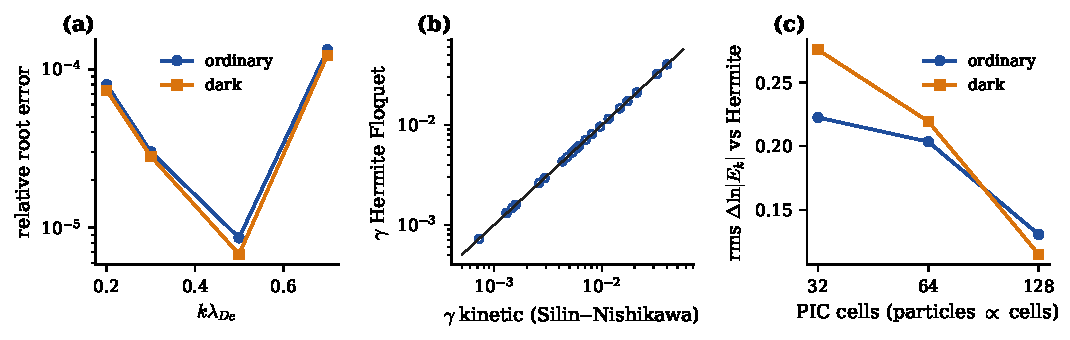
\includegraphics[width=\linewidth]{figures/fig_verification.pdf}
\caption{Verification. (a) Relative error of the fitted complex frequency against the independent kinetic root, ordinary and dark ($\eta=0.3$), $N_n=128$, $N_x=8$. (b) Hermite Floquet growth rate against the kinetic dipole-pump relation of Silin (sideband determinant, see text). (c) RMS difference of $\ln|E_k|$ between Dark-JAX-in-Cell and Hermite on $2\le\wpe t\le12$ for Landau damping, for increasing cells and particles.}\label{fig:verify}
\end{figure*}

\subsection{The Hermite truncation instability and the certified windows}
The method has one limit that matters for the rest of the paper. In a non-uniform field the truncated AW Galerkin operator $-v\partial_x+(q/m)E\partial_v$ is not anti-self-adjoint; its frozen-field spectrum has growing modes in the top third of the Hermite ladder, with a rate that rises with $N_n$ (Fig.~\ref{fig:aw}a; at $K=5$, $N_n=128$, $E_1=10^{-2}$ the largest growth rate is \awEigAW, against $\le\awEigSW$ for the symmetric basis, which is neutral to round-off). This is a numerical instability of the basis, not physics. It is distinct from the physical OTSI, which the Hermite model reproduces and which amplifies finite-$k$ fields strongly at resonance (the Hermite model understates the growth: Nn 32/64/128 agree with each other and end 1.3--4 times below the exact solution). The AW instability is excited by the large-amplitude pump and ends the simulation by loss of positivity or by the step budget.

A \emph{certified window} is defined by checks declared before the runs: refinement pairs ($N_x$, $N_n$, closure strength) must agree to 10\,\% in $\Delta K_e$ and $\Wext$, the electron distribution must stay positive ($K_s>0$ and $k=0$ $T_x>0$), the solver must reach the time, and the energy ledger must close. The window is the minimum of these times. It is therefore a lower bound on where the Hermite results can be trusted, not a statement about physics.

\begin{figure*}[t]
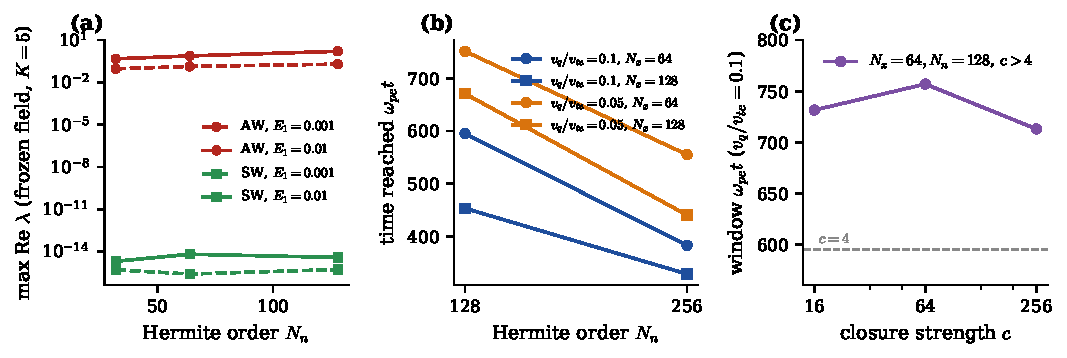
\includegraphics[width=\linewidth]{figures/fig_aw.pdf}
\caption{The limit of the method. (a) Largest real part of the frozen-field spectrum for the AW basis (grows with $N_n$) and the symmetric-weight basis (round-off), $K=5$. (b) Time reached by AW runs with closure $c=4$ at $\vq=0.1$ and $0.05$ for $N_x=64,128$ and $N_n=128,256$, all ended at the step budget inside the instability: more resolution ends the run sooner. (c) At $\vq=0.1$, $N_x=64$, $N_n=128$ a stronger fixed closure extends the window from 595 to a ceiling of 713--757.}\label{fig:aw}
\end{figure*}

Alternatives were tested and rejected, all under pre-declared gates (Table~\ref{tab:failed}). Higher resolution on GPU ($N_x\in\{64,128\}$, $N_n\in\{128,256\}$, $\vq=0.1$ and $0.05$) failed the declared window-extension check and ended every run inside the instability at \gpuWinA--\gpuWinB\ ($\vq=0.1$) and \gpuWinC--\gpuWinD\ ($\vq=0.05$): the pairs agree to the end of the shorter run, so this is a failure of the resolution route rather than a disagreement. In a frozen field no closure strength up to 1024 brings the AW growth below $10^{-3}$ at peak field $4\times10^{-3}$ (39/39 points fail), leaving a floor that grows as $K^{0.15}N_n^{0.30}E^{1.26}$, so a resolution-consistent closure strength does not exist for this closure family. A stable Galerkin form of Dai~\cite{Dai2026} is unstable in the AW coordinates in float64 at $N_n\ge64$ (the AW-to-orthonormal change of basis has condition $\sim2^N$) but stable and accurate against the kinetic OTSI relation in symmetric Hermite functions of width $a/\sqrt2$; the symmetric-weight basis itself, and the anti-symmetric square-root form of Issan et al.~\cite{Issan2024a,Issan2025}, are linearly neutral to round-off and accurate against the same relation, but were rejected under their declared nonlinear $\vq=0.1$ gates (symmetric weight: every run blows up at $t=637$--738 and the refinement pair agrees only to 634; square-root form: departure from the grid reference at 391 and 498, earlier than the symmetric weight). Production therefore stays with the AW basis and the field-scaled closure, and the windows below are its windows.

\begin{table*}[t]
\caption{Negative and amended results that bound the claims. ``Declared'' means the check was committed before the run and not amended.}\label{tab:failed}
\small
\begin{tabular}{@{}L{3.1cm}L{4.3cm}L{5.0cm}L{4.0cm}@{}}\toprule
Study & Check & Outcome & Consequence\\\midrule
GPU resolution extension & Longer window at higher resolution, $\vq=0.1$, 0.05 & Failed; every run ends at the step budget inside the instability & No new window; a stable basis is needed\\
Closure-strength route & AW growth below $10^{-3}$ in a frozen field for some closure strength & Failed; a floor remains & Scaled-closure option not built\\
Stiffness vs.\ instability & Which eigenvalue limits the step & Stiff eigenvalue is the closure; the instability (max Re $\lambda=2$--3) is not & Integrator is not the limit\\
Lawson factor (closure) & Step reduction at $c=4$ & Failed as declared (no gain) & Useful for $c=64$ only\\
Lawson factor (streaming) & Step reduction with an exact streaming factor & Failed & Rejected\\
Dai / symmetric weight / square root & Declared nonlinear gates at $\vq=0.1$ & Failed (Sec.~\ref{sec:verify}) & AW basis with closure stays\\
Finite coherence, first version & Declared phase variance & Wrong: realized $\tau_c$ was $2\times$ nominal & Corrected version declared and used\\
Seed deficit hypothesis & ``Homogeneous truncation effect'' & Rejected & Deficit is seed back-reaction\\
Collisional steady-state check & Window longer than the record & Declaration defect; declared follow-up used, deviation from $P_{\rm ss}$ $3\times10^{-5}$ & Follow-up result used\\
Collisions, 5\,\% agreement & Kinetic equals linear within 5\,\% & \rtwoKtwo\ of \rtwoKtwoN\ pass; six detuned cases at $\nu_{ei}=10^{-3}$ fail & Seed effect; seed-scale follow-up passed\\
Earlier collision pilot & Restart-chunk length; ion heating & Failed as declared ($T_i$ responds to the halved exchange) & Recorded, not amended\\
Collision-form controls & Several declared checks & Mis-specified or at round-off level & Recorded; ledger closes to $10^{-17}$\\\bottomrule
\end{tabular}
\end{table*}

\section{Finite reservoir and finite coherence}\label{sec:r1}
\subsection{Design}
Two idealizations of the prescribed-drive calculation are removed. First, in the self-consistent mode the dark photon is a free $k=0$ Proca mode with $\Omega_D=\omega_L$ whose energy reservoir $U_{D0}$ is finite and is depleted by the transfer; we use $u=U_{D0}/(\nTV)=0.1,1,10$ with $\eta$ chosen so that the initial effective force matches the prescribed drive. Second, the dark field has a finite coherence time: the prescribed drive is $E_0\cos(\omega_Lt+\Phi(t))$ with $\Phi$ a phase random walk of independent Gaussian frequency samples, giving a Lorentzian line of half-width $1/\tau_c$ and no phase resets. The comparison is always with the exact linear law for the same drive (and, for the reservoir, the linear coupled oscillator $(\bar E,\bar J,E_D,A_D)$, whose matrix exponential agrees with an ODE solver to $6.6\times10^{-11}$).

\subsection{Windows at each drive}
\begin{table*}[t]
\caption{Certified windows for the strong-drive set-up with closure $c=64$ integrated exactly. Members: $(N_x,N_n)=(32,64),(64,64),(32,128),(64,128)$ and $(32,64)$ at $c=32$. The window is the minimum of refinement-pair times, positivity times, times reached and the cap $T=1000$; the grid column is the masked spectral-grid reference (reported, not part of the window).}\label{tab:windows}
\tabWindows
\end{table*}
Table~\ref{tab:windows} gives the windows: \winA, \winB\ and \winC\ for $\vq=0.03$, 0.05 and 0.07. The windows are set by positivity loss of the $N_x=64$ members, that is, by the AW truncation instability reaching the resolved range, not by disagreement of the refinement pairs. The strongest certified drive is $\vq=0.07$ with window \winC. Drives above that, including $\vq=0.1$, have no window beyond about 760 (Sec.~\ref{sec:verify}).

\subsection{Linear transfer and the seed back-reaction}
At $\vq=0.07$ the work $\Wext$ follows the exact linear resonant law over the whole window (Fig.~\ref{fig:r1}a): the maximum of $|\Wext/\Wlin-1|$ over four resolutions is \rnlBound\,\%, the four members agree on it to \rnlSpread, and at the window end $\Wext=\rnlWext$ against $\Wlin=\rnlWlin$ (in $\nTV$). The mean-field frequency shift, measured as the slope of the lock-in phase difference, is at most \rnlDw\ $\wpe$ (the declared resolution threshold was $10^{-3}\omega_L$; not resolved). No saturation and no detuning are resolved. The departure rule (a $10\,\%$ departure in the coarsest member confirmed at $5\,\%$ in all refinements) is not met.

The residual deficit is not a drive effect. At the three drives it is the same to three digits (it grows as $-10^{-8}\,t^2$) until the OTSI stage, ending at \dEndA, \dEndB\ and \dEndC\,\% at the window ends. A seed-scale test at $\vq=0.07$ (the initial density fluctuations multiplied by $s$) shows the deficit scales as $s^2$ (Table~\ref{tab:seed}, Fig.~\ref{fig:r1}b): the ratio of $s=0.1$ to $s=1$ is \fuRatio\ and the unseeded run gives \fuDc\ at $\wpe t=400$. The deficit is therefore the back-reaction of the quiver-advected seed modulation on the mean field (the $\langle\delta n\,\delta E\rangle$ term of the mean-field identity), set by the imposed fluctuation level, not by the pump. A physical fluctuation level different from $5\times10^{-4}$ would rescale it. Our earlier hypothesis that it is a truncation effect of the seedless homogeneous system was tested and rejected: the unseeded deficit is only \fuFtwo\ of the seeded one. Only the seed scales $0$, $0.1$ and $1$ at $t\le400$ were run.

\begin{table*}[t]
\caption{Seed-scale test of the deficit $D=\Wext/\Wlin-1$ at $\vq=0.07$, $N_x=32$, $N_n=64$ ; the seed amplitudes are multiplied by $s$.}\label{tab:seed}
\small
\tabSeed
\end{table*}

\begin{figure*}[t]
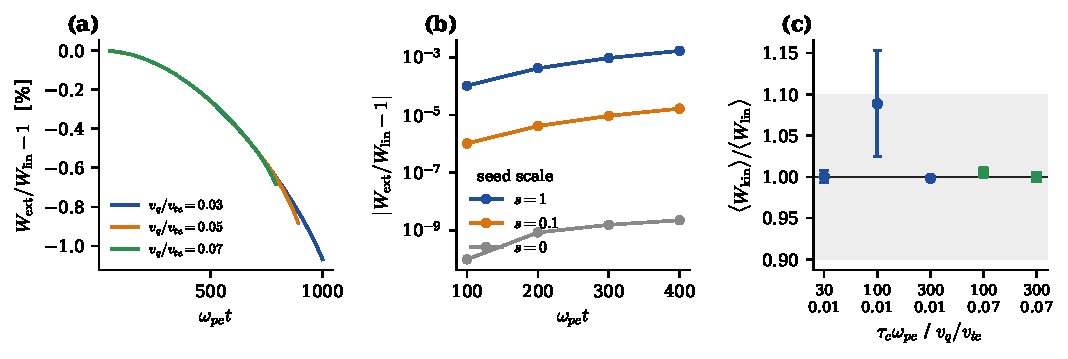
\includegraphics[width=\linewidth]{figures/fig_r1.pdf}
\caption{Finite reservoir and coherence. (a) $\Wext/\Wlin-1$ for the $N_x=32$, $N_n=64$ member at the three drives, each to its certified window; the three curves coincide until the OTSI stage. (b) The deficit at $\vq=0.07$ for seed scales $s=1$, $0.1$, 0. (c) Finite coherence: ensemble ratio $\langle W_{\rm kin}\rangle/\langle W_{\rm lin}\rangle$ with standard error over six realizations for $\tau_c\wpe=30,100,300$ at $\vq=0.01$ (window 1000) and $100,300$ at $\vq=0.07$ (window \winC); band: $\pm10\,\%$.}\label{fig:r1}
\end{figure*}

\subsection{Energetics and the onset of the OTSI}
Why the transfer stays linear is energetic. At the window end of $\vq=0.07$, \rnlDKe\ of the $\Wext=\rnlWext\,\nTV$ resides in coherent $k=0$ electron quiver kinetic energy; the ions receive \rnlIonShare\,\% of $\Wext$. The energy of the $k\ne0$ electron motion is small and oscillating: with the mean flow removed it sloshes between wave kinetic and field energy with a period of about 67\,$\wpe^{-1}$ near the onset, so a single time sample is not a heating measure; the average over $200\,\wpe^{-1}$ (the HHS filter, Sec.~\ref{sec:hhs}) is \hhsDErEndC\ initial thermal energies at the end of the window. The fluctuating-field amplitude ($\sum_{k\ge1}|E_k|^2$) reaches about \rnlFluct\,$E_0^2$ only when the OTSI turns on, at $\wpe t=\rnlOtsi$ ($N_x=32$) to \rnlOtsiN\ (higher $N_x$ and $N_n$ members; onset defined in the gates, compared within equal $N_x$). After that the run ends by positivity loss. Within the window the instability has not extracted a resolvable fraction of the work. \emph{This is the main limitation of the bound}: it says that no saturation appears \emph{before} the cascade of fluctuations starts, and nothing about what happens after.

\subsection{Finite reservoir}
In the self-consistent mode (Table~\ref{tab:reservoir}) the dark energy $U_D(t)$ follows the linear coupled-oscillator prediction at all three drives: within \rOneDev\,$U_{D0}$ (maximum over six cases, $u=0.1,1,10$) at $\vq=0.01$ and $0.03$ over the windows 1000 and 940, and within \rnlResO\,\% and \rnlResOZ\,\% of $U_{D0}$ at $\vq=0.07$ for $u=1$ and 10 over the window \winC. The beat times equal $\pi/\eta$ ($\eta=\rnlEtaO$ and $\rnlEtaOZ$ for $u=1,10$). The accumulated work $W_D$ follows the matched prescribed drive until the split time $t_{\rm split}=\rnlSplitO$ and $\rnlSplitOZ$ (equal to the linear values): the reservoir gives up \rnlWDfrac\,\% of its energy for $u=1$ and exchanges energy through beats for $u=10$, with $W_D$ within \rnlResWO\,\% and \rnlResWOZ\,\% of the linear prediction while it is above 20\,\% of its running maximum. Finite reservoir depletion is therefore captured by the linear theory; no nonlinear reservoir response is resolved. The ledger closes to \rnlLedger\ over all \rnlNruns\ runs of the strong-drive study (declared bound $10^{-6}$).
\begin{table*}[t]
\caption{Finite reservoir (self-consistent dark field, $\Omega_D=\omega_L$), $\vq=0.07$.}\label{tab:reservoir}
\small
\begin{tabular}{@{}lcccc@{}}\toprule
$u=U_{D0}/\nTV$ & $\eta$ & max $|U_D-U_D^{\rm lin}|/U_{D0}$ [\%] & $t_{\rm split}$ & $W_D$ bound [\%]\\\midrule
1 & \rnlEtaO & \rnlResO & \rnlSplitO & \rnlResWO\\
10 & \rnlEtaOZ & \rnlResOZ & \rnlSplitOZ & \rnlResWOZ\\\bottomrule
\end{tabular}
\end{table*}

\subsection{Finite coherence}
Figure~\ref{fig:r1}c shows the ensemble ratio of the kinetic to the linear same-drive work. At $\vq=0.01$ (window 1000, with $\tau_c$ the field coherence time) the ratios are $\cohRHZ\pm\cohSeHZ$, $\cohROZZ\pm\cohSeOZZ$ and $\cohRHZZ\pm\cohSeHZZ$ for $\tau_c\wpe=30,100,300$; the value at $\tau_c\wpe=100$ is 1.4 standard errors above unity and is consistent with the sampling spread of six realizations. At $\vq=0.07$ the ratios are $\rnlROZZ\pm\rnlRseOZZ$ and $\rnlRHZZ\pm\rnlRseHZZ$ for $\tau_c\wpe=100$, 300, with bounds on the ensemble nonlinear correction (including twice the standard error) of \rnlRbOZZ\,\% and \rnlRbHZZ\,\%; individual realizations deviate more (up to \rnlRmaxOZZ\,\% and \rnlRmaxHZZ\,\% of the peak linear work), with ratios on both sides of unity. The late work rate saturates at about $E_0^2\tau_c\omega_L^2/4$ instead of growing, as in the linear theory. The first coherence runs realized a phase variance $dt/\tau_c$ rather than the declared $2\,dt/\tau_c$, i.e. a coherence time twice the nominal; the records were kept and relabelled and a corrected version was declared and run (Table~\ref{tab:failed}).

\subsection{Scope of the reservoir and coherence bounds}
The bounds hold for one box ($L=40$), one ion mass, $T_i=T_e$, drives up to $\vq=0.07$, windows set by the AW instability, fluctuation seeds of one amplitude ($5\times10^{-4}$), a Lorentzian line only, and reservoir and coherence not combined in one run. Not done: a Gaussian line, windows beyond about 790 at 0.07, $\vq>0.07$ and inhomogeneous dark fields. The grid reference (masked spectral grid) agrees with the Hermite coarse member until 870 and 863 at $\vq=0.07$ (Table~\ref{tab:windows}).

\section{Collisional absorption}\label{sec:r2}
\subsection{Linear drag law}
With collisions the uniform relative velocity relaxes at the Morse rate, identical in LBO-EM and LBO-G ($\beta=0$),
\begin{equation}
\nu_{\rm eff}=\frac{\nu_{ei}}{2}\Big(1+\frac{m_e}{m_i}\Big),
\end{equation}
so the uniform driven cold response obeys $\dot J=\omega_L^2(\bar E+E_D)-\nu_{\rm eff}J$ and the steady absorbed power per volume is
\begin{align}
P_{\rm ss}&=\frac{\omega_L^2\,\nu_{\rm eff}\,\omega^2E_0^2}{2\left[(\omega_L^2-\omega^2)^2+\nu_{\rm eff}^2\omega^2\right]},\\
P_{\rm ss}^{\rm res}&=\frac{\omega_L^2E_0^2}{2\nu_{\rm eff}},
\end{align}
with the transient decaying as $\exp(-\nu_{\rm eff}t/2)$ (1/e time $4/\nu_{ei}$). This is the cold Drude response of Dubovsky and Hern\'andez-Chifflet~\cite{DubovskyHC2015}, who write the friction as $-m_e\nu(u_e-u_i)$ with a Spitzer-like $\nu$ and find a shielding suppression $\propto m^2/\omega_p^2$ off resonance; and it matches the non-resonant absorption rate of McDermott and Witte~\cite{McDermottWitte2020}. Their $\nu$ corresponds to $\nu_{\rm eff}$ here. In our model $\nu$ is \emph{constant}: the Spitzer scaling $\nu\propto T_e^{-3/2}$ is absent.

\subsection{Design and gates}
The set-up is that of the strong-drive study (mobile ions, pump frame, $c=64$ with Lawson, $T=1000$) with Dougherty $e$--$e$, $e$--$i$ and $i$--$i$ collisions in both conventions. The grid is $\vq=0.01,0.03,0.05$ by $\nu_{ei}=10^{-3},3\times10^{-3},10^{-2},3\times10^{-2}$ by $\omega=\omega_L,0.9,1.1$ (in $\wpe$): 192 runs in all, including $N_x=64$ and $N_n=128$ refinement members and unseeded controls. Checks were declared before the runs. Every LBO-EM case reaches $t=1000$ with refinement pairs agreeing to the end and a refinement spread of the late rate $\le2.2\times10^{-4}$. The nonrelativistic window ($T_e/T_e(0)<90$, i.e. $v_{te}<0.3c$) is shorter only for $\vq=0.05$ resonant. Rates are evaluated at $t_b=996.5$.

\subsection{Kinetic against linear}
\begin{table*}[t]
\caption{Late-time absorbed power, kinetic ($N_x=32$, $N_n=64$, LBO-EM) against the exact transient-inclusive linear law, $\vq=0.03$. $T_e/T_e(0)$ at $t_b$; last column: kinetic equals linear within 5\,\%.}\label{tab:r2}
\small
\tabRtwo
\end{table*}
Table~\ref{tab:r2} and Fig.~\ref{fig:r2} give the result. Where collisions act and the linear transient has decayed, the kinetic absorption equals the linear drag law: at $\nu_{ei}=3\times10^{-2}$ the late rate is within \rtwoPss\,\% of $P_{\rm ss}$ for all three frequencies and drives, and the steady-state law holds in \rtwoKthree\ of \rtwoKthreeN\ cases where $P_{\rm lin}$ is within 10\,\% of $P_{\rm ss}$. For the other cases the kinetic rate equals the exact \emph{transient-inclusive} linear law to 5\,\% except in six cases, but the steady state is not reached within $t=1000$: for $\nu_{ei}=10^{-3},3\times10^{-3},10^{-2}$ the resonant rate is only 0.20, 0.48, 0.89 of $P_{\rm ss}$ (the amplitude transient has 1/e time $4/\nu_{ei}$). The sustained law is therefore tested directly at $\nu_{ei}=3\times10^{-2}$ (and $10^{-2}$ detuned), and through the linear ODE for the rest. The 5\,\% agreement check passes in \rtwoKtwo\ of \rtwoKtwoN\ cases.

The six failures are the detuned $\nu_{ei}=10^{-3}$ cases, where the kinetic late rate is $8$--$14\,\%$ high (mean $+\rtwoDetL\,\%$ at 0.9 and $+\rtwoDetH\,\%$ at 1.1), independent of $\vq$. In the unseeded controls the kinetic and linear laws agree to $3\times10^{-8}$, and a seed-scale follow-up (declared after the main analysis and before its runs) shows the departure scales as $s^2$ (ratios \rtwoFuA\ and \rtwoFuB\ for $s=0.1$, against $s^2=0.01$): it is the same seed back-reaction as for the strong-drive study, large only where $\Wext$ is itself tiny. The resonant late rate is low by $1.5$--$4\,\%$ at $\nu_{ei}=10^{-3}$ (\rtwoResLo\ at the lowest) and by $\le0.2\,\%$ at $3\times10^{-2}$; at $\vq=0.05$ resonant the deficit (3.7\,\%) is larger than at 0.01 and 0.03, but drive amplitude and heating are not separable in these data, so a few-percent heating or drive correction is allowed but not attributed.

\begin{figure*}[t]
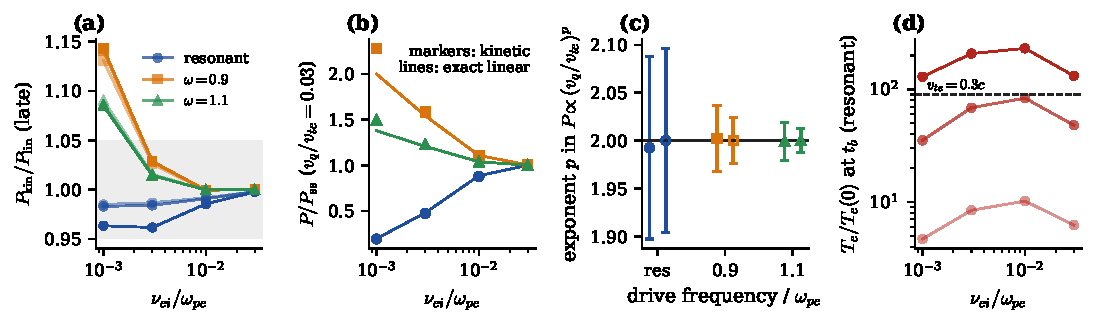
\includegraphics[width=\linewidth]{figures/fig_r2.pdf}
\caption{Collisional absorption. (a) Ratio of the kinetic to the exact linear late-time power for $\vq=0.01,0.03,0.05$ (increasing opacity) and three drive frequencies; band: the 5\,\% gate. (b) Late power relative to the steady state $P_{\rm ss}$ at $\vq=0.03$, kinetic (markers) and linear (lines). (c) Fitted exponent $p$ of the drive amplitude, kinetic (filled) and linear (open), with standard errors; the solid line marks $p=2$. (d) Electron heating at $t_b$ for the resonant cases, same opacity code as (a); dashed: $v_{te}=0.3c$, beyond which the nonrelativistic model is outside its validity.}\label{fig:r2}
\end{figure*}

\subsection{Deposition law}
Fitting $\ln P=a+p\ln(\vq)+q\ln\nu_{ei}$ over the 12 cases per frequency (standard errors from the residual scatter, so they include the transient-state curvature) gives for resonant, 0.9 and 1.1: $p=\rtwoPR\pm\rtwoPeR$, $\rtwoPL\pm\rtwoPeL$, $\rtwoPH\pm\rtwoPeH$ (kinetic), against 2 (linear, exact), and $q=\rtwoQR\pm\rtwoQeR$, $\rtwoQL\pm\rtwoQeL$, $\rtwoQH\pm\rtwoQeH$ (kinetic) against $\rtwoQlR$, $\rtwoQlL$, $\rtwoQlH$ (linear). The amplitude scaling is quadratic. The $\nu_{ei}$ scaling follows the transient-inclusive linear law, not a pure power: the detuned rate grows with $\nu$ (off-resonant absorption proportional to $\nu$, until the beat transient decays), and the resonant rate falls with $\nu$ with an exponent near $-1/2$ because the steady state is not reached. The geometric-mean correction of kinetic to linear power is $\kappa=\rtwoKR\pm\rtwoKeR$, $\rtwoKL\pm\rtwoKeL$, $\rtwoKH\pm\rtwoKeH$. The domain of the law is $\vq\le0.05$, $\nu_{ei}\in[10^{-3},3\times10^{-2}]\wpe$, $\omega\in\{0.9,\omega_L,1.1\}\wpe$, $t\le1000$, one box and mass ratio, one seed level.

\subsection{Collision form and heating}
EM and G ($\beta=0$) agree in $\Wext$ to \rtwoCVwx\ and the late-rate ratio differs by $\le7\times10^{-6}$ (agreement checks pass in \rtwoCV\ of \rtwoCVN\ cases); electron kinetic energy and temperature differ by $\le8\times10^{-3}$. Ion temperature differs by up to 31\,\% and the electron--ion energy exchange is halved, as expected: the absorption is set by the momentum friction, identical in the two forms, while the exchange is the temperature-difference rate. The ion-heating check of the earlier pilot failed as declared for this reason (Table~\ref{tab:failed}). Electron heating is large: $T_e/T_e(0)$ reaches \rtwoTmax\ (Fig.~\ref{fig:r2}d), beyond $v_{te}=0.3c$ for $T_e/T_e(0)>90$, i.e.\ outside the nonrelativistic model. Heating does not change the rate in this model because $\nu$ is constant ($R_{\rm late}$ stays within 1\,\% of unity while $T_e/T_e(0)$ rises from 7 to 70 at $\vq=0.03$, $\nu_{ei}=10^{-2}$, resonant). Ion heating is small ($T_i/T_i(0)\le2.8$) and the $e\to i$ exchange is $4\times10^{-5}$ to $1.6\times10^{-2}$ of $\Wext$, growing in proportion to $\nu_{ei}$. The steady-state self-check of the linear theory had a declaration defect; its declared follow-up passes (Table~\ref{tab:failed}).

\subsection{What is needed for a cosmological statement}
Our collisions fix $\nu$ at a constant. A cosmological deposition law needs (i) the velocity-dependent Coulomb frequency $\nu(T_e)\propto T_e^{-3/2}$, which couples the heating to the absorption and lowers it; (ii) radiative and Compton cooling; (iii) cosmological expansion and ionization history; (iv) relativistic electrons, since $T_e/T_e(0)$ exceeds the nonrelativistic limit; (v) the $k\ne0$ coupling of a real dark-photon field; and (vi) a steady-state measurement at $\nu_{ei}\le10^{-2}$ resonant, which needs $t\gg4/\nu_{ei}$. $\nu_{ee}$ and $\nu_{ii}$ are order-of-magnitude choices that do not enter the uniform drag.

\section{Discussion}\label{sec:discussion}
\paragraph*{What the results do establish.} Within a one-dimensional, nonrelativistic, deterministic-seed model with the ingredients of HHS, and for the drives and times listed in Table~\ref{tab:windows}, the energy transfer from a uniform resonant drive follows the linear resonant law: $\vq=0.03$ to $\wpe t=1000$, 0.05 to \winB\ and 0.07 to \winC. At the strongest drive the nonlinear correction to $\Wext$ is bounded by \rnlBound\,\%, and the work has reached $\Wext=\rnlWext\,\nTV$ (\wextA, \wextB\ and \wextC\ $\nTV$ at the window ends for 0.03, 0.05, 0.07), almost all of it coherent $k=0$ quiver energy. A finite reservoir and a finite coherence time of $\tau_c\omega_{pe}\ge100$ do not change this. Collisions give the linear Drude law, with the kinetic rate equal to the linear law to a few per cent and to \rtwoPss\,\% at steady state.

\paragraph*{The nonrelativistic limitation.} The model is nonrelativistic: the Vlasov equation uses the Newtonian momentum and the kinetic-energy ledger the quadratic form. This matters for the quantities reported here. The coherent $k=0$ quiver energy at the window end, $\Wext\simeq\wextA$, \wextB\ and \wextC\ $\nTV$ for $\vq=0.03$, 0.05, 0.07, corresponds to an electron speed $\sqrt{2\Wext/(n m_e)}$ of \quivA$c$, \quivB$c$ and \quivC$c$ (nonrelativistic formula), so that for most of every window the quiver is beyond the range in which Newtonian dynamics is accurate, and the electron temperature in the collisional runs reaches $v_{te}>0.3c$ (Fig.~\ref{fig:r2}d). Relativistic mass increase lowers the plasma frequency of the quivering electrons by a fraction of the order of $v^2/c^2$, which for $v\gtrsim0.2c$ exceeds the resonance width $\sim1/(\wpe t)$ of the driven oscillator long before the end of our windows. A relativistic model would therefore detune the resonance, and could saturate the transfer by that mechanism alone, independently of the nonlinear plasma processes that HHS invoke. Our linear-law result is thus a statement about the nonrelativistic model; it is not a statement about the relativistic plasma, and it cannot be compared with a relativistic PIC run beyond the time at which the quiver speed is small ($\wpe t\lesssim200$ at $\vq=0.03$). We have not run a relativistic model, and this is the largest untested difference from HHS (Sec.~\ref{sec:hhs}).

\paragraph*{What they do not establish.} (i) The growth of higher-$k$ fluctuations by the strong pump, which in our model is the OTSI (we take this to be the process described in the HHS abstract; that identification is our reading, not something we tested against their simulations), has its onset at $\wpe t\simeq\rnlOtsi$--\rnlOtsiN\ at $\vq=0.07$, at the end of our window. The windows end by positivity loss at nearly the same times, because the numerical instability of the Hermite basis reaches the resolved range there, so we cannot say whether the transfer would saturate after the cascade develops. The bound is a statement about the interval before it. In our runs about \rnlCohShare\,\% of the transferred energy is still coherent $k=0$ quiver energy at the window end. HHS do not count that coherent part as deposited (their Figs.~2 and 3 show the $k\ne0$ kinetic energy), so the large $\Wext$ is not comparable to their saturation level; what is comparable is stated in Sec.~\ref{sec:hhs}. For the claim at times after the cascade, ours is neither a confirmation nor a refutation. (ii) The model is one-dimensional (and nonrelativistic, above), with a box $L=40\,c/\wpe$ and the strict $2/3$ mask retaining Fourier modes $k\le9$ at $N_x=32$ and $k\le20$ at $N_x=64$ (in units of $2\pi/L$), against 1000 cells in HHS; the retained modes cover the onset but not a developed spectrum. (iii) The seed amplitude is imposed; at this seed the deficit is \rnlBound\,\%, and a different fluctuation level rescales it. (iv) Drives above $\vq=0.07$ (including $\vq=0.1$) have no window beyond about 760, so the claims are bounds for $\vq\le0.07$ and $\wpe t\lesssim790$ at the strongest drive, and nothing more.

\paragraph*{Why a nonlinear detuning could be expected.} The trapping time of O'Neil~\cite{ONeil1965}, $\tau=(m/eEk)^{1/2}$, ends linear theory, and the ponderomotive coupling is the origin of the modulational and collapse processes of Zakharov~\cite{Zakharov1972}. For the uniform pump the mean-field law is exact and neither matters until finite-$k$ fluctuations grow, which is why the first deviations in our model are those of the finite-$k$ OTSI.

\subsection{Comparison with the HHS simulations}\label{sec:hhs}
\paragraph*{What HHS plot.} The energy ``$\Delta E/n_em_e$'' of their Figs.~2 and 3 is the change of the thermal energy density $n_\alpha m_\alpha v_{th}^2/2$ of each species (SM Eqs.~S35 and S36), with $v_{th}^2$ the one-dimensional ($x$) velocity variance about the mean; SM footnote~8 states that the plotted temperatures measure the total kinetic energy of electrons and ions with the $k=0$ component removed, and that energy already thermalized cannot be told apart from energy in $k\ne0$ oscillations. The coherent $k=0$ quiver energy is therefore \emph{not} counted as deposited; the mean field enters separately as $\langle E^2\rangle/2$ (red solid line). The temperature is a global (box) variance, not a local one. All curves are filtered with a moving average over $200\,\wpe^{-1}$ (Fig.~2 caption). Their statement that the deposited energy is about the initial thermal energy ($5\times10^{-4}\,n_em_ec^2$ for $v_{th}^2=10^{-3}c^2$) is a statement about this $k\ne0$ energy. In Sec.~II of the SM the particle number per cell is raised for weak drives so that the shot-noise energy equals the driven energy at $\wpe t\approx2.4$ (SM Eq.~S38), and the driven energy is converted into incoherent $k\ne0$ noise within $\wpe t\simeq3$--4 (SM Sec.~II).

\paragraph*{Same definition here.} Our records carry the box-mean-flow-subtracted one-dimensional electron variance, $\Delta E=\tfrac12m_e\Delta(M_{xx}-M_x^2/n)$, and the mean field $\bar E$; the figure script evaluates both with the trailing $200\,\wpe^{-1}$ average. The definition is therefore the same as theirs, one-dimensional, global, with the $k=0$ mean flow removed.

\paragraph*{What is comparable.} Only the resonant $\vq=0.03$ case is: same drive, $T_e$, mass ratio, box, filter and definition, and our window ($\wpe t\le1000$) covers the time over which their top panel of Fig.~2 saturates ($\wpe t\lesssim500$; SM Sec.~III notes the loss of resonance at about 800). Table~\ref{tab:hhs} compares the numbers; the HHS entries are read off their logarithmic plot (accuracy about a factor of 1.5). Their weak case, $v_q/v_{te}=10^{-3}$, saturates at $\wpe t\simeq1500$--2300, beyond our windows, and we have no run at that drive; their Landau--Zener runs (Fig.~3) and their $T_e/T_i$ histories to $\wpe t=8\times10^4$ (SM Fig.~S3) have no counterpart here; our $\vq=0.05$ and 0.07 are not drives they show, and we did not run those in their model.
\begin{table*}[t]
\caption{Resonant drive $\vq=0.03$: HHS (PRL Fig.~2, top; values read off the plot) against this work ($N_x=32$, $N_n=64$). $\Delta E_e$: change of the one-dimensional $k\ne0$ electron kinetic energy; $\bar E^2/2$: mean-field energy ($\langle E^2\rangle/2$ for HHS); both in units of $n_em_ec^2$ with the $200\,\wpe^{-1}$ trailing average; $E_{\rm th}=5\times10^{-4}$.}\label{tab:hhs}
\small
\begin{tabular}{@{}lccc@{}}\toprule
 & HHS & ours, $\wpe t=500$ & ours, $\wpe t=1000$\\\midrule
$\Delta E_e$ & $\approx2.5\times10^{-2}$ ($\approx50\,E_{\rm th}$) & \hhsDEVZZA\ (\hhsDErVZZA\,$E_{\rm th}$) & \hhsDEEndA\ (\hhsDErEndA\,$E_{\rm th}$)\\
$\bar E^2/2$ & $\approx10^{-3}$ at 800, $\lesssim10^{-4}$ at 1000 & \hhsFldVZZA\ (linear \hhsFldLinVZZA) & \hhsFldEndA\ (linear \hhsFldLinEndA)\\\bottomrule
\end{tabular}
\end{table*}

\paragraph*{Reading.} At this matched drive and over the time in which HHS see the $k\ne0$ energy rise to about fifty initial thermal energies and the field energy collapse, our electron $k\ne0$ energy is \hhsDErVZZA\ initial thermal energies at $\wpe t=500$ and \hhsDErEndA\ at 1000, and the mean-field energy follows the linear law to \hhsFldRatioA\ of it. We therefore do not reproduce their saturation at $\vq=0.03$. We do not conclude that their result is wrong; the model differs in ways we have not tested: (a) the loading and the seed level (our deterministic seed has relative amplitude $5\times10^{-4}$; theirs is shot noise set by the particle number, with the noise equal to the driven energy at $\wpe t\approx2.4$); (b) our Fourier truncation retains $k\le1.4\,\wpe/c$ at $N_x=32$ and $\le3.1$ at $N_x=64$, i.e. $k\lambda_{De}\le0.045$ and $0.1$, whereas their instabilities populate wavenumbers up to $\lambda_{De}^{-1}$ (SM Sec.~III); (c) their pusher is relativistic, and the accumulated quiver speed $v_q^D\wpe t/2$ reaches about \quivAtTZZ$c$ by $\wpe t\approx200$ and \quivAtVZZ$c$ by 500 (\quivA$c$ at 1000 from our work ledger), so that the relativistic frequency shift, of the order of $v^2/c^2$, can exceed the resonance width $\sim1/t$ well before their saturation time; our model has no such shift. We regard (c) as the most likely single cause of the difference at $\vq=0.03$, but this is a hypothesis: we have not run a relativistic model, and items (b) and (c) can only be settled by runs we have not done. Our numbers at $\vq=0.05$ and 0.07 are bounds in this model and are not comparable to any HHS figure.

\section{Conclusions}
We built and verified a noise-free Hermite--Fourier solver for the canonical Maxwell--Proca--Vlasov system. Its limit is a numerical truncation instability of the asymmetrically weighted Hermite basis, which bounds certified windows to \winA, \winB\ and \winC\ at $\vq=0.03$, 0.05, 0.07; no higher resolution, stronger closure, or alternative basis we tried (Dai, symmetric weight, square-root form) removes it. Inside those windows, the energy transfer follows the linear resonant law to \rnlBound\,\%, with no resolved frequency detuning, finite dark-reservoir depletion and finite coherence follow the linear predictions, and the small deficit is seed back-reaction. With collisions, the absorption is the linear Drude law with $\nu_{\rm eff}=(\nu_{ei}/2)(1+m_e/m_i)$, quadratic in the drive, and independent of the collision form. These are bounds in a restricted model. They do not test nonlinear suppression after the oscillating two-stream cascade develops, relativistic electrons (the coherent quiver speed reaches \quivA$c$ at $\vq=0.03$ and \quivC$c$ at $\vq=0.07$ within the windows, so the relativistic detuning of the resonance is the main open difference from HHS), $k\ne0$ coupling, or a temperature-dependent collision frequency; a stable basis is needed to extend the windows.

\section*{Data and code availability}
All code, records and generated results are in the Dark-SPECTRAX repository~\cite{DarkSPECTRAX} (\url{https://github.com/uwplasma/Dark-SPECTRAX}). The records and study scripts are those of commit \texttt{a3ef7a6} of the \texttt{main} branch; the manuscript, figures and number macros are in \texttt{paper/} at the commit that follows it (stated in \texttt{paper/README.md}). No release or tag has been made. Figures, tables and quoted numbers are generated from the records by \texttt{paper/make\_figures.py}; the record index below maps each figure and table to its files. The parent solver SPECTRAX~\cite{SPECTRAX} was used at the commits stored in the records: \texttt{3de6b2b} (finite reservoir and coherence), \texttt{4090fbe} (strong-drive study) and \texttt{35231ab} (collisions; the pin in \texttt{pyproject.toml}); the branch tip at the time of writing is \texttt{729d7fe}. These commits belong to the \texttt{integration/dark-baseline} branch of SPECTRAX, an unmerged integration branch that collects open parent pull requests with the features used here (field-scaled closure, Lawson factor, collision conventions); it is not a release. Checks were committed in \texttt{studies/r1\_common.py}, \texttt{r1nl\_gates.py} and \texttt{r2\_gates.py} before the runs.

{\raggedright\emph{Record index} (paths relative to the repository root). Fig.~\ref{fig:verify} and Table~\ref{tab:verify}: \texttt{docs/\_static/b00/run.json}, \texttt{studies/instab/otsi.json}, \texttt{studies/c05/run.json}, \texttt{studies/gpures/c08.json}, \texttt{studies/c09/run.json} (summary in \texttt{docs/results.md}). Fig.~\ref{fig:aw}: \texttt{studies/highk/eig.json}, \texttt{studies/gpures/summary.json}, \texttt{studies/rclosure/stagef.json}. Tables~\ref{tab:windows} and~\ref{tab:reservoir}, Fig.~\ref{fig:r1}a: \texttt{studies/r1nl/stage1\_summary.json} and \texttt{stage2\_summary.json}. Table~\ref{tab:seed} and Fig.~\ref{fig:r1}b: \texttt{studies/r1nl/followup\_summary.json}. Fig.~\ref{fig:r1}c and the weak-drive reservoir runs: \texttt{studies/r1/coherence2\_summary.json}, \texttt{studies/r1/reservoir\_summary.json}. Table~\ref{tab:r2} and Fig.~\ref{fig:r2}: \texttt{studies/r2/summary.json}. Table~\ref{tab:hhs}: \texttt{studies/r1nl/runs}. Failed and amended checks (Table~\ref{tab:failed}): \texttt{docs/status.md}.\par}

\begin{acknowledgments}
[Acknowledgments to be completed by the author.]
\end{acknowledgments}

% Numbers typed in the text that are not macros (source: docs/results.md, generated from records by docs/make_results.py):
%  Landau window / O'Neil / etc. are not quoted. 6.6e-11 matrix exponential vs ODE: R1 section (a); 5.17/nu_e, 5e-10, 2.7x cost: stiffdiag,
%  expint, stream sections; 1.3-4x Hermite understatement: "Physical: broadband finite-k instability" table; 1024, 39/39, K^0.15 Nn^0.30 E^1.26:
%  rclosure section; 637-738, 634, 391, 498: SW and antisym sections; 3.7%, 1.5-4%, <=0.2%, 7->70, T_i<=2.8, 4e-5..1.6e-2: R2 reading;
%  3e-8 unseeded controls, 3e-5 T0b, <=7e-6, 8e-3, 31%: R2 gates and reading; 15 v_te, 1e-9: H00 table; 2e-5 echo, 1e-13 Dougherty, 1e-3 Weibel/B08,
%  2-15% adjoint, 2e-13/5e-10 AD: B01/B06, B11, B09, B08, C09 sections; 0.20/0.48/0.89 resonant P/Pss: R2 table (f_ss column).
\bibliography{refs}
\end{document}
